\documentclass[9pt,a4paper]{article}
\usepackage[margin=1.8cm,top=2.0cm,bottom=2.0cm]{geometry}
\usepackage{booktabs,colortbl,xcolor,array,makecell,hhline}
\usepackage{amsmath,amssymb}
\usepackage{helvet}\renewcommand{\familydefault}{\sfdefault}
\usepackage{fancyhdr,graphicx}
\usepackage[colorlinks=true,linkcolor=primary,urlcolor=primary,
            bookmarks=true,pdfborder={0 0 0}]{hyperref}
\usepackage{parskip,enumitem,titlesec,needspace}
\setlength{\parskip}{2pt}
\definecolor{passgreen}{RGB}{198,239,206}
\definecolor{failred}{RGB}{255,199,206}
\definecolor{warnamber}{RGB}{255,235,156}
\definecolor{r2green}{RGB}{198,239,206}
\definecolor{r2amber}{RGB}{255,235,156}
\definecolor{primary}{RGB}{0,70,127}
\definecolor{sepgray}{RGB}{130,130,130}
\titleformat{\section}{\normalsize\bfseries\color{primary}}{}{0em}{}
            [\vspace{-4pt}\textcolor{primary}{\rule{\linewidth}{0.5pt}}]
\titlespacing{\section}{0pt}{16pt}{6pt}
\newcommand{\exhead}[1]{%
  \medskip\noindent{\small\bfseries\color{primary}#1}%
  \par\vspace{-5pt}\noindent\textcolor{primary}{\rule{\linewidth}{0.4pt}}\vspace{2pt}}
\pagestyle{fancy}\fancyhf{}
\lhead{\small\textcolor{primary}{\textbf{Surrogate Factory}}}
\chead{\small\textcolor{sepgray}{CONFIDENTIAL}}
\rhead{\small\textcolor{primary}{UCFATIGUE\_1}}
\lfoot{\small\textcolor{sepgray}{Surrogate Factory v2.2 --- Automated Validation Report}}
\rfoot{\small\thepage}
\renewcommand{\headrulewidth}{0.4pt}\renewcommand{\footrulewidth}{0.4pt}
\begin{document}
% ==== EXECUTIVE SUMMARY ====
\thispagestyle{fancy}

\begin{center}
  {\large\bfseries\color{primary} Executive Summary --- Surrogate Model Validation Report}\\[2pt]
  {\small\color{sepgray} Use case: \textbf{UCFATIGUE\_1} \quad|\quad 09 September 2026 \quad|\quad 2 model(s)}
\end{center}
\vspace{-4pt}\noindent\rule{\linewidth}{1pt}\vspace{3pt}

\begin{center}
\colorbox{warnamber}{\begin{minipage}{0.66\linewidth}
  \vspace{5pt}\centering
  {\normalsize\bfseries REQUIREMENTS PARTIALLY MET}\\[4pt]
  {\small\bfseries Recommended model:} {\small GradientBoosting}\\[5pt]
\colorbox{r2green}{\begin{minipage}{0.97\linewidth}\vspace{2pt}\centering {\small\bfseries Avg R\textsuperscript{2}: 0.9643} \enspace---\enspace {\small Excellent}\vspace{2pt}\end{minipage}}\\[2pt]
\colorbox{warnamber}{\begin{minipage}{0.97\linewidth}\vspace{2pt}\centering {\small\bfseries Q90 Accuracy} \enspace---\enspace {\small Partially met}\\[1pt]{\footnotesize Pass: 1g, Vertical maneuver, Vertical gust, Turn, n0}\\[1pt]{\footnotesize\color{red} Fail: Frontal gust, Giro}\vspace{2pt}\end{minipage}}
  \vspace{5pt}
\end{minipage}}
\end{center}

\section{Project Overview}
\renewcommand{\arraystretch}{1.2}
\begin{tabular}{|l|p{0.60\linewidth}|}
  \hline
  \textbf{Use case}           & UCFATIGUE\_1 \\ \hline
  \textbf{Inputs}             & FLAP, Altitude, TAS, Mass, q, gamma, Type\_segment, Xcg(\%CMA) \\ \hline
  \textbf{Outputs}            & 7: 1g, Vertical maneuver, Vertical gust, Turn, Frontal gust, n0, Giro \\ \hline
  \textbf{Train / Val / Test} & 80\% / 10\% / 10\% \\ \hline
  \textbf{Accuracy target}    & Q90 $<$ 10\% relative error per output \\ \hline
\end{tabular}

\par\begin{minipage}{\linewidth}
\section{Variable Correlation --- Input vs Output}
\begin{center}
\includegraphics[width=0.80\linewidth,height=0.46\textheight,keepaspectratio]{analysis_plots/data_scatter_vars.png}\end{center}
\end{minipage}\par\medskip
\section{Data Statistics}
Per-variable statistics over all data (train + val + test), as \texttt{Train\_set.describe()} reports them in the feature-selection notebook: count, mean, standard deviation, minimum, quartiles and maximum.

\par\begin{minipage}{\linewidth}
\exhead{Inputs}
\begin{center}
\footnotesize
\renewcommand{\arraystretch}{1.15}
\resizebox{\linewidth}{!}{%
\begin{tabular}{|l|r|r|r|r|r|r|r|r|}
\hline
\textbf{} & \textbf{count} & \textbf{mean} & \textbf{std} & \textbf{min} & \textbf{P25} & \textbf{P50} & \textbf{P75} & \textbf{max} \\ \hline
\textbf{FLAP} & 869 & 2.2186 & 5.3696 & 0 & 0 & 0 & 0 & 23 \\ \hline
\textbf{Altitude} & 869 & 9294.6341 & 7701.9019 & 18 & 2,000 & 8,000 & 15,000 & 26,000 \\ \hline
\textbf{TAS} & 869 & 190.871 & 48.8676 & 101 & 144 & 197.5712 & 230 & 302 \\ \hline
\textbf{Mass} & 869 & 18874.7779 & 1324.6887 & 14,125 & 17,761 & 18,905 & 19,991 & 21,886 \\ \hline
\textbf{q} & 869 & 4510.2453 & 1845.3166 & 1652.3866 & 2881.2026 & 3579.9882 & 6375.4631 & 9637.8604 \\ \hline
\textbf{gamma} & 869 & -0.2667 & 4.5734 & -39.4508 & -4.7042 & 0 & 2.9442 & 18.2194 \\ \hline
\textbf{Xcg(\%CMA)} & 869 & 19.4107 & 4.0946 & 14.6 & 16.43 & 18.5 & 20.58 & 29.3 \\ \hline
\end{tabular}
}
\par\vspace{2pt}
{\scriptsize Input variables — Train\_set.describe()}
\end{center}
\end{minipage}\par\medskip
\par\begin{minipage}{\linewidth}
\exhead{Outputs}
\begin{center}
\footnotesize
\renewcommand{\arraystretch}{1.15}
\resizebox{\linewidth}{!}{%
\begin{tabular}{|l|r|r|r|r|r|r|r|r|}
\hline
\textbf{} & \textbf{count} & \textbf{mean} & \textbf{std} & \textbf{min} & \textbf{P25} & \textbf{P50} & \textbf{P75} & \textbf{max} \\ \hline
\textbf{1g} & 869 & 53.6228 & 8.2962 & 31.561 & 47.364 & 51.778 & 61.558 & 73.308 \\ \hline
\textbf{Vertical maneuver} & 869 & 19.1377 & 2.4542 & 12.031 & 17.185 & 18.893 & 21.394 & 24.471 \\ \hline
\textbf{Vertical gust} & 869 & 0.6494 & 0.1681 & 0.3466 & 0.5097 & 0.575 & 0.806 & 1.092 \\ \hline
\textbf{Turn} & 869 & 6.3621 & 0.6415 & 4.122 & 6.01 & 6.382 & 6.83 & 7.53 \\ \hline
\textbf{Frontal gust} & 869 & 0.4806 & 1.1541 & 0 & 0 & 0 & 0 & 3.722 \\ \hline
\textbf{n0} & 869 & 1.9391 & 0.0777 & 1.73 & 1.9 & 1.94 & 1.98 & 2.19 \\ \hline
\textbf{Giro} & 869 & 1.9959 & 1.5329 & 0.662 & 1.299 & 1.587 & 1.874 & 7.599 \\ \hline
\end{tabular}
}
\par\vspace{2pt}
{\scriptsize Output variables — Train\_set.describe()}
\end{center}
\end{minipage}\par\medskip
\section{Model Selection}
\begin{minipage}{\linewidth}
\renewcommand{\arraystretch}{1.2}
\begin{tabular}{|l|r|r|r|}
  \hline
  \textbf{Model} & \textbf{Avg R\textsuperscript{2}} & \textbf{Q90 pass (7)} & \textbf{KS pass (7)} \\ \hline
  { MLP} & { 0.5237} & { 5/7} & { 7/7} \\ \hline
  {\bfseries GradientBoosting\ $\star$} & {\bfseries 0.9643} & {\bfseries 5/7} & {\bfseries 2/7} \\ \hline
\end{tabular}
\par\vspace{4pt}
{\footnotesize $\star$ Recommended model.\enspace Q90 target: $<10\%$.\enspace KS: $p\geq 0.05$ = no overfitting.}
\end{minipage}

\section{Accuracy Assessment (Q90 \& R\textsuperscript{2})}
\begin{minipage}{\linewidth}
\renewcommand{\arraystretch}{1.2}
\begin{tabular}{l|rrr|rrr|}
  \hline
  \textbf{Output} & \multicolumn{3}{c|}{\textbf{MLP}} & \multicolumn{3}{c|}{\textbf{GradientBoosting}\ $\star$} \\ \hline
  & R\textsuperscript{2} & Q90 & Gap & R\textsuperscript{2} & Q90 & Gap \\ \hline
  1g & \cellcolor{r2amber}0.9160 & \cellcolor{passgreen}0.0473 & \cellcolor{passgreen}-0.0527 & \cellcolor{r2green}0.9797 & \cellcolor{passgreen}0.0257 & \cellcolor{passgreen}-0.0743 \\ \hline
  Vertical maneuver & \cellcolor{r2amber}0.9116 & \cellcolor{passgreen}0.0554 & \cellcolor{passgreen}-0.0446 & \cellcolor{r2green}0.9723 & \cellcolor{passgreen}0.0318 & \cellcolor{passgreen}-0.0682 \\ \hline
  Vertical gust & \cellcolor{r2amber}0.9377 & \cellcolor{passgreen}0.0918 & \cellcolor{passgreen}-0.0082 & \cellcolor{r2green}0.9914 & \cellcolor{passgreen}0.0262 & \cellcolor{passgreen}-0.0738 \\ \hline
  Turn & \cellcolor{failred}0.7544 & \cellcolor{passgreen}0.0783 & \cellcolor{passgreen}-0.0217 & \cellcolor{r2amber}0.9286 & \cellcolor{passgreen}0.0351 & \cellcolor{passgreen}-0.0649 \\ \hline
  Frontal gust & \cellcolor{r2green}0.9794 & \cellcolor{failred}11.3300 & \cellcolor{failred}+11.2300 & \cellcolor{r2green}0.9964 & \cellcolor{failred}0.2795 & \cellcolor{failred}+0.1795 \\ \hline
  n0 & \cellcolor{failred}-0.7292 & \cellcolor{passgreen}0.0723 & \cellcolor{passgreen}-0.0277 & \cellcolor{r2amber}0.9317 & \cellcolor{passgreen}0.0149 & \cellcolor{passgreen}-0.0851 \\ \hline
  Giro & \cellcolor{failred}-0.1042 & \cellcolor{failred}0.9005 & \cellcolor{failred}+0.8005 & \cellcolor{r2amber}0.9499 & \cellcolor{failred}0.2215 & \cellcolor{failred}+0.1215 \\ \hline
\end{tabular}
\par\vspace{4pt}
{\footnotesize \colorbox{r2green}{\ } R\textsuperscript{2}$\!\geq\!0.95$\enspace \colorbox{r2amber}{\ } R\textsuperscript{2}$\!\in[0.80,0.95)$\enspace \colorbox{failred}{\ } R\textsuperscript{2}$\!<\!0.80$ or Q90 fail\enspace \colorbox{passgreen}{\ } pass\enspace Gap$=$Q90$-$target ($<\!0\Rightarrow$ margin)}
\end{minipage}

\par\begin{minipage}{\linewidth}
\section{Training History}
\begin{center}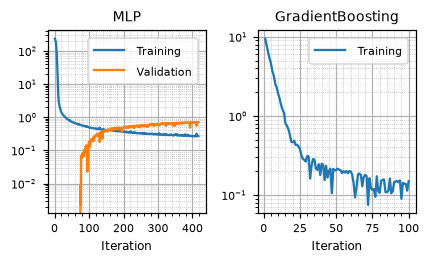
\includegraphics[width=0.70\linewidth,height=0.28\textheight,keepaspectratio]{../training_curve.png}\end{center}
{\footnotesize Training and validation loss per iteration, log scale. The validation curve is measured, not approximated: per epoch on the early-stopping split for the MLP, per stage on the validation split for gradient boosting (whose training curve is its per-stage deviance). Models saved before this was recorded fall back to the $(1-R^2)\cdot\mathrm{Var}(y)/2$ approximation.}\end{minipage}\par\medskip

\par\begin{minipage}{\linewidth}
\section{Predicted vs True --- GradientBoosting}
\begin{center}
\includegraphics[width=\linewidth,height=0.80\textheight,keepaspectratio]{analysis_plots/winner_pred_true.png}\end{center}
\end{minipage}\par\medskip


\section{Data Split Quality}
\begin{minipage}{\linewidth}
\renewcommand{\arraystretch}{1.2}
\begin{tabular}{|l|r|c|}
  \hline\textbf{Metric} & \textbf{Value} & \textbf{Pass} \\ \hline
  Residual voxel proportion ($\leq\!0.05$) & 0.000 & \cellcolor{passgreen}$\checkmark$ \\ \hline
  Valid test proportion & 0.931 & \\ \hline
  p-hacking test proportion ($\leq\!0.05$ warn) & 0.006 & \cellcolor{passgreen}$\checkmark$ \\ \hline
  Isolated test proportion ($\leq\!0.05$ warn) & 0.063 & \cellcolor{failred}$\times$ \\ \hline
  Chi\textsuperscript{2} p-value ($\geq\!0.05$) & 0.7969 & \cellcolor{passgreen}$\checkmark$ \\ \hline
\end{tabular}
\end{minipage}
\textcolor{passgreen!60!black}{\textbf{No p-hacking concern:}} only 0.6\% of test points lie closer to a training point than training points are to each other, so the test error is not flattered. \textcolor{failred!70!black}{\textbf{Isolated points:}} 6.3\% of test points have no training point nearby, so part of the test error measures extrapolation rather than interpolation --- the model may look worse there than it is in the region it was trained on.

\section{Overfitting Check (KS Test) --- GradientBoosting}
\begin{minipage}{\linewidth}
\renewcommand{\arraystretch}{1.15}
\begin{tabular}{|l|r|}
  \hline\textbf{Output} & \textbf{KS p-value} \\ \hline
  1g & \cellcolor{failred}0.004 \\ \hline
  Vertical maneuver & \cellcolor{passgreen}0.161 \\ \hline
  Vertical gust & \cellcolor{failred}0.042 \\ \hline
  Turn & \cellcolor{failred}0.044 \\ \hline
  Frontal gust & \cellcolor{passgreen}0.974 \\ \hline
  n0 & \cellcolor{failred}0.032 \\ \hline
  Giro & \cellcolor{failred}0.017 \\ \hline
\end{tabular}
\par\vspace{4pt}
{\footnotesize \colorbox{passgreen}{\ } $p\geq 0.05$ --- no overfitting\enspace \colorbox{failred}{\ } $p<0.05$ --- overfitting detected}
\end{minipage}
\clearpage
\thispagestyle{empty}
\vspace*{\fill}
\begin{center}
  \textcolor{sepgray}{\rule{0.40\linewidth}{1pt}}\\[20pt]
  {\Huge\bfseries\color{primary} Deep Analysis}\\[10pt]
  {\large\color{sepgray} UCFATIGUE\_1}\\[6pt]
  {\normalsize\color{sepgray} Winner Model --- Full Validation}\\[20pt]
  \textcolor{sepgray}{\rule{0.40\linewidth}{1pt}}
\end{center}
\vspace*{\fill}
\clearpage
% ==== PART 3 - DEEP ANALYSIS ====
\label{sec:deepanalysis}
\begin{center}
  {\normalsize\bfseries\color{primary} Deep Analysis --- GradientBoosting}\\[2pt]
  {\small\color{sepgray} Mirrors \texttt{validation\_template.ipynb} --- all computations from validation CSVs}
\end{center}
\vspace{4pt}
\begin{itemize}[leftmargin=2em,itemsep=1pt,topsep=2pt]
  \item \hyperref[sec:d1]{3.1 Data Overview}
  \item \hyperref[sec:d2]{3.2 Train-Test Split Analysis}
  \item \hyperref[sec:d3]{3.3 Error Quantification --- P(E)}
  \item \hyperref[sec:d4]{3.4 P(E|X) --- Error Conditional on Inputs}
  \item \hyperref[sec:d5]{3.5 P(E|Y) --- Error Conditional on Outputs}
  \item \hyperref[sec:d6]{3.6 Uncertainty Analysis}
\end{itemize}

\clearpage
\section{Data Overview}
\label{sec:d1}

Statistical summary of inputs and outputs over all data (train + val + test), as reported by \texttt{describe()} in the feature-selection notebook: count, mean, standard deviation, minimum, quartiles and maximum per variable. All figures in this part are drawn by \texttt{validationlib}, matching the extended validation notebook.

\exhead{Input Statistics}
\begin{center}
\footnotesize
\renewcommand{\arraystretch}{1.15}
\resizebox{\linewidth}{!}{%
\begin{tabular}{|l|r|r|r|r|r|r|r|r|}
\hline
\textbf{} & \textbf{count} & \textbf{mean} & \textbf{std} & \textbf{min} & \textbf{P25} & \textbf{P50} & \textbf{P75} & \textbf{max} \\ \hline
\textbf{FLAP} & 869 & 2.2186 & 5.3696 & 0 & 0 & 0 & 0 & 23 \\ \hline
\textbf{Altitude} & 869 & 9294.6341 & 7701.9019 & 18 & 2,000 & 8,000 & 15,000 & 26,000 \\ \hline
\textbf{TAS} & 869 & 190.871 & 48.8676 & 101 & 144 & 197.5712 & 230 & 302 \\ \hline
\textbf{Mass} & 869 & 18874.7779 & 1324.6887 & 14,125 & 17,761 & 18,905 & 19,991 & 21,886 \\ \hline
\textbf{q} & 869 & 4510.2453 & 1845.3166 & 1652.3866 & 2881.2026 & 3579.9882 & 6375.4631 & 9637.8604 \\ \hline
\textbf{gamma} & 869 & -0.2667 & 4.5734 & -39.4508 & -4.7042 & 0 & 2.9442 & 18.2194 \\ \hline
\textbf{Xcg(\%CMA)} & 869 & 19.4107 & 4.0946 & 14.6 & 16.43 & 18.5 & 20.58 & 29.3 \\ \hline
\end{tabular}
}
\par\vspace{2pt}
{\scriptsize Input variables — Train\_set.describe()}
\end{center}
\par\begin{minipage}{\linewidth}
\exhead{Input Histograms}
\begin{center}
\includegraphics[width=1.0\linewidth,height=0.80\textheight,keepaspectratio]{analysis_plots/data_input_hist.png}\end{center}
\end{minipage}\par\medskip
\par\begin{minipage}{\linewidth}
\exhead{Input Cumulative Distributions}
\begin{center}
\includegraphics[width=1.0\linewidth,height=0.80\textheight,keepaspectratio]{analysis_plots/data_input_cdf.png}\end{center}
\end{minipage}\par\medskip
\exhead{Output Statistics}
\begin{center}
\footnotesize
\renewcommand{\arraystretch}{1.15}
\resizebox{\linewidth}{!}{%
\begin{tabular}{|l|r|r|r|r|r|r|r|r|}
\hline
\textbf{} & \textbf{count} & \textbf{mean} & \textbf{std} & \textbf{min} & \textbf{P25} & \textbf{P50} & \textbf{P75} & \textbf{max} \\ \hline
\textbf{1g} & 869 & 53.6228 & 8.2962 & 31.561 & 47.364 & 51.778 & 61.558 & 73.308 \\ \hline
\textbf{Vertical maneuver} & 869 & 19.1377 & 2.4542 & 12.031 & 17.185 & 18.893 & 21.394 & 24.471 \\ \hline
\textbf{Vertical gust} & 869 & 0.6494 & 0.1681 & 0.3466 & 0.5097 & 0.575 & 0.806 & 1.092 \\ \hline
\textbf{Turn} & 869 & 6.3621 & 0.6415 & 4.122 & 6.01 & 6.382 & 6.83 & 7.53 \\ \hline
\textbf{Frontal gust} & 869 & 0.4806 & 1.1541 & 0 & 0 & 0 & 0 & 3.722 \\ \hline
\textbf{n0} & 869 & 1.9391 & 0.0777 & 1.73 & 1.9 & 1.94 & 1.98 & 2.19 \\ \hline
\textbf{Giro} & 869 & 1.9959 & 1.5329 & 0.662 & 1.299 & 1.587 & 1.874 & 7.599 \\ \hline
\end{tabular}
}
\par\vspace{2pt}
{\scriptsize Output variables — Train\_set.describe()}
\end{center}
\par\begin{minipage}{\linewidth}
\exhead{Output Histograms}
\begin{center}
\includegraphics[width=1.0\linewidth,height=0.80\textheight,keepaspectratio]{analysis_plots/data_output_hist.png}\end{center}
\end{minipage}\par\medskip
\par\begin{minipage}{\linewidth}
\exhead{Output Cumulative Distributions}
\begin{center}
\includegraphics[width=1.0\linewidth,height=0.80\textheight,keepaspectratio]{analysis_plots/data_output_cdf.png}\end{center}
\end{minipage}\par\medskip
\clearpage
\section{Train-Test Split Analysis}
\label{sec:d2}

A well-designed split produces training and test distributions that are similar but not identical. The Kolmogorov-Smirnov (KS) test and the Anderson-Darling (AD) test are used to assess distributional similarity. $H_0$: both sets come from the same distribution. $p<0.05$ rejects $H_0$ (undesirable if too low; undesirable if the split was done by stratification and $p$ is too high).

\par\begin{minipage}{\linewidth}
\exhead{Output Distributions: Train vs Test}
\begin{center}
\includegraphics[width=1.0\linewidth,height=0.80\textheight,keepaspectratio]{analysis_plots/split_output_dists.png}\end{center}
\end{minipage}\par\medskip
\par\begin{minipage}{\linewidth}
\exhead{Input Distributions: Train vs Test}
\begin{center}
\includegraphics[width=1.0\linewidth,height=0.80\textheight,keepaspectratio]{analysis_plots/split_input_dists.png}\end{center}
\end{minipage}\par\medskip
\exhead{KS and AD Test Results}
\begin{center}
\footnotesize
\renewcommand{\arraystretch}{1.15}
\begin{tabular}{|l|r|r|}
\hline
\textbf{} & \textbf{KS} & \textbf{AD} \\ \hline
\textbf{1g} & \cellcolor{passgreen}0.126 & \cellcolor{passgreen}0.1656 \\ \hline
\textbf{Vertical maneuver} & \cellcolor{passgreen}0.9577 & \cellcolor{passgreen}0.25 \\ \hline
\textbf{Vertical gust} & \cellcolor{passgreen}0.4768 & \cellcolor{passgreen}0.25 \\ \hline
\textbf{Turn} & \cellcolor{passgreen}0.4441 & \cellcolor{passgreen}0.1512 \\ \hline
\textbf{Frontal gust} & \cellcolor{passgreen}1 & \cellcolor{passgreen}0.25 \\ \hline
\textbf{n0} & \cellcolor{passgreen}0.7097 & \cellcolor{passgreen}0.25 \\ \hline
\textbf{Giro} & \cellcolor{passgreen}0.4079 & \cellcolor{passgreen}0.25 \\ \hline
\end{tabular}
\par\vspace{2pt}
{\scriptsize Train vs test p-values. Red: $p<0.05$ (distributions differ).}
\end{center}
\exhead{Split Quality --- Voxel Tesselation Proximity (p-hacking check)}
Beyond matching distributions, a split can still flatter the model if test points sit right next to training points (\textbf{p-hacking}) or probe regions the model never saw (\textbf{isolated}, \textbf{residual voxel}). The VTPM method from \texttt{validationlib} (SF\_9 cell 9.0) classifies every test point.

\begin{minipage}{\linewidth}
\renewcommand{\arraystretch}{1.2}
\begin{tabular}{|l|r|c|}
  \hline\textbf{Metric} & \textbf{Value} & \textbf{Pass} \\ \hline
  Residual voxel proportion ($\leq\!0.05$) & 0.000 & \cellcolor{passgreen}$\checkmark$ \\ \hline
  Valid test proportion & 0.931 & \\ \hline
  p-hacking test proportion ($\leq\!0.05$ warn) & 0.006 & \cellcolor{passgreen}$\checkmark$ \\ \hline
  Isolated test proportion ($\leq\!0.05$ warn) & 0.063 & \cellcolor{failred}$\times$ \\ \hline
  Chi\textsuperscript{2} p-value ($\geq\!0.05$) & 0.7969 & \cellcolor{passgreen}$\checkmark$ \\ \hline
\end{tabular}
\end{minipage}

\textcolor{passgreen!60!black}{\textbf{No p-hacking concern:}} only 0.6\% of test points lie closer to a training point than training points are to each other, so the test error is not flattered. \textcolor{failred!70!black}{\textbf{Isolated points:}} 6.3\% of test points have no training point nearby, so part of the test error measures extrapolation rather than interpolation --- the model may look worse there than it is in the region it was trained on.

\par\begin{minipage}{\linewidth}
\exhead{Error Distribution: Valid vs Isolated Test Points}
Same comparison for the test points with no training neighbour.
\begin{center}
\includegraphics[width=1.0\linewidth,height=0.80\textheight,keepaspectratio]{analysis_plots/isolated_hist.png}\end{center}
\begin{center}
\footnotesize
\renewcommand{\arraystretch}{1.15}
\begin{tabular}{|l|r|r|r|}
\hline
\textbf{} & \textbf{AD} & \textbf{KS} & \textbf{KW} \\ \hline
\textbf{1g} & \cellcolor{failred}0.001 & \cellcolor{failred}3.19e-07 & \cellcolor{failred}3.36e-06 \\ \hline
\textbf{Vertical maneuver} & \cellcolor{failred}0.001 & \cellcolor{failred}1e-05 & \cellcolor{failred}9.16e-05 \\ \hline
\textbf{Vertical gust} & \cellcolor{failred}0.001 & \cellcolor{failred}0.000205 & \cellcolor{failred}9.84e-06 \\ \hline
\textbf{Turn} & \cellcolor{failred}0.001 & \cellcolor{failred}0.0015 & \cellcolor{failred}0.000255 \\ \hline
\textbf{Frontal gust} & \cellcolor{failred}0.0016 & \cellcolor{passgreen}0.0605 & \cellcolor{failred}0.0069 \\ \hline
\textbf{n0} & \cellcolor{failred}0.001 & \cellcolor{failred}9.08e-06 & \cellcolor{failred}9.59e-06 \\ \hline
\textbf{Giro} & \cellcolor{failred}0.001 & \cellcolor{failred}8.38e-05 & \cellcolor{failred}0.000123 \\ \hline
\end{tabular}
\par\vspace{2pt}
{\scriptsize Valid ($n=160$) vs Isolated ($n=14$) absolute-error distributions, on a subsample of the test set. Red: $p<0.05$ (the flagged points behave differently).}
\end{center}
\end{minipage}\par\medskip
\clearpage
\section{Error Quantification --- P(E)}
\label{sec:d3}

Two error metrics are studied:
\begin{itemize}[leftmargin=1.4em,itemsep=1pt,topsep=1pt]
  \item \textbf{Residue:} $e_i = y_i - \hat{y}_i$. A centred ($\mu\approx 0$), symmetric distribution indicates an unbiased model.
  \item \textbf{Absolute Error:} $|e_i|$. Always non-negative; its Q90 must satisfy the accuracy requirement.
\end{itemize}

\exhead{Residue Statistics Table}
Bootstrap confidence bounds shown as superscript (upper) and subscript (lower).
\begin{center}
\footnotesize
\renewcommand{\arraystretch}{1.15}
\resizebox{\linewidth}{!}{%
\begin{tabular}{|l|r|r|r|r|r|r|r|r|r|r|r|r|r|r|r|}
\hline
\textbf{} & \textbf{count} & \textbf{min} & \textbf{max} & \textbf{mean} & \textbf{(BS)mean} & \textbf{median} & \textbf{(BS)median} & \textbf{std} & \textbf{(BS)std} & \textbf{IQR} & \textbf{(BS)IQR} & \textbf{kurtosis} & \textbf{(BS)kurtosis} & \textbf{skewness} & \textbf{(BS)skewness} \\ \hline
\textbf{1g} & 174 & -9.66 & 1.97 & -0.21 & $^{-0.058}_{-0.391}$ & -0.0456 & $^{0.0052}_{-0.145}$ & 1.16 & $^{1.65}_{0.712}$ & 0.594 & $^{0.711}_{0.405}$ & 29.2 & $^{39}_{4.75}$ & -4.36 & $^{-0.99}_{-5.12}$ \\ \hline
\textbf{Vertical maneuver} & 174 & -2.39 & 1.85 & -0.0341 & $^{0.0198}_{-0.0985}$ & -0.0074 & $^{0.0187}_{-0.0344}$ & 0.419 & $^{0.543}_{0.299}$ & 0.224 & $^{0.272}_{0.194}$ & 10.8 & $^{18.2}_{5.26}$ & -1.61 & $^{0.518}_{-2.96}$ \\ \hline
\textbf{Vertical gust} & 174 & -0.127 & 0.0307 & -0.0024 & $^{-0.00021}_{-0.0049}$ & -0.0013 & $^{0.000259}_{-0.0026}$ & 0.0157 & $^{0.0208}_{0.0102}$ & 0.0097 & $^{0.0126}_{0.0086}$ & 23.7 & $^{31.9}_{3.58}$ & -3.64 & $^{-0.587}_{-4.47}$ \\ \hline
\textbf{Turn} & 174 & -0.84 & 0.881 & -0.0176 & $^{0.0053}_{-0.038}$ & -0.0031 & $^{0.0162}_{-0.0146}$ & 0.184 & $^{0.231}_{0.137}$ & 0.0983 & $^{0.127}_{0.0784}$ & 8 & $^{13.1}_{4.4}$ & -0.788 & $^{1.16}_{-2.23}$ \\ \hline
\textbf{Frontal gust} & 174 & -0.249 & 0.628 & 0.0061 & $^{0.0162}_{-0.0034}$ & 9.16e-05 & $^{\text{9.16e-05}}_{\text{9.16e-05}}$ & 0.068 & $^{0.104}_{0.0304}$ & 1.39e-17 & $^{\text{1.38e-05}}_{0}$ & 48.3 & $^{74.6}_{16.4}$ & 5.57 & $^{7.88}_{-3.53}$ \\ \hline
\textbf{n0} & 174 & -0.0583 & 0.0883 & 0.0022 & $^{0.0042}_{-0.001}$ & 0.0014 & $^{0.0028}_{-0.0016}$ & 0.0192 & $^{0.0236}_{0.0149}$ & 0.015 & $^{0.0199}_{0.0123}$ & 4.62 & $^{6.99}_{1.23}$ & 0.979 & $^{1.72}_{-0.55}$ \\ \hline
\textbf{Giro} & 174 & -1.55 & 1.51 & -0.034 & $^{0.0073}_{-0.083}$ & -0.0113 & $^{-0.0023}_{-0.024}$ & 0.308 & $^{0.381}_{0.223}$ & 0.142 & $^{0.181}_{0.0916}$ & 11.1 & $^{16.7}_{5.09}$ & -0.253 & $^{2.2}_{-2.57}$ \\ \hline
\end{tabular}
}
\par\vspace{2pt}
{\scriptsize Residue statistics with bootstrap confidence intervals (superscript/subscript bounds).}
\end{center}
\exhead{Absolute Error Statistics Table}
\begin{center}
\footnotesize
\renewcommand{\arraystretch}{1.15}
\resizebox{\linewidth}{!}{%
\begin{tabular}{|l|r|r|r|r|r|r|r|r|r|r|r|r|r|r|r|}
\hline
\textbf{} & \textbf{count} & \textbf{min} & \textbf{max} & \textbf{mean} & \textbf{(BS)mean} & \textbf{median} & \textbf{(BS)median} & \textbf{std} & \textbf{(BS)std} & \textbf{IQR} & \textbf{(BS)IQR} & \textbf{kurtosis} & \textbf{(BS)kurtosis} & \textbf{skewness} & \textbf{(BS)skewness} \\ \hline
\textbf{1g} & 174 & 0.0028 & 9.66 & 0.572 & $^{0.704}_{0.422}$ & 0.246 & $^{0.388}_{0.223}$ & 1.03 & $^{1.48}_{0.483}$ & 0.55 & $^{0.668}_{0.412}$ & 39.7 & $^{56.8}_{7.16}$ & 5.57 & $^{6.65}_{2.44}$ \\ \hline
\textbf{Vertical maneuver} & 174 & 0.000887 & 2.39 & 0.229 & $^{0.286}_{0.183}$ & 0.113 & $^{0.135}_{0.0918}$ & 0.353 & $^{0.456}_{0.249}$ & 0.177 & $^{0.281}_{0.135}$ & 13.9 & $^{21.9}_{6.48}$ & 3.45 & $^{4.14}_{2.5}$ \\ \hline
\textbf{Vertical gust} & 174 & 3.12e-05 & 0.127 & 0.0088 & $^{0.0107}_{0.0074}$ & 0.0055 & $^{0.0062}_{0.0044}$ & 0.0132 & $^{0.0182}_{0.0082}$ & 0.0073 & $^{0.0092}_{0.0064}$ & 38.1 & $^{52.7}_{7.83}$ & 5.28 & $^{6.28}_{2.52}$ \\ \hline
\textbf{Turn} & 174 & 0.0016 & 0.881 & 0.105 & $^{0.123}_{0.0815}$ & 0.0513 & $^{0.0602}_{0.0367}$ & 0.153 & $^{0.183}_{0.103}$ & 0.0955 & $^{0.135}_{0.0681}$ & 9.81 & $^{18.5}_{5.81}$ & 3 & $^{3.75}_{2.44}$ \\ \hline
\textbf{Frontal gust} & 174 & 9.16e-05 & 0.628 & 0.0162 & $^{0.0267}_{0.0079}$ & 9.16e-05 & $^{\text{9.16e-05}}_{\text{9.16e-05}}$ & 0.0663 & $^{0.0932}_{0.0298}$ & 0.002 & $^{0.0042}_{0.000267}$ & 49.2 & $^{88.6}_{14.8}$ & 6.54 & $^{8.71}_{3.9}$ \\ \hline
\textbf{n0} & 174 & 5.6e-05 & 0.0883 & 0.013 & $^{0.0155}_{0.0115}$ & 0.0076 & $^{0.0096}_{0.006}$ & 0.0143 & $^{0.0177}_{0.011}$ & 0.0141 & $^{0.0189}_{0.0114}$ & 8.74 & $^{12.5}_{1.89}$ & 2.52 & $^{2.95}_{1.39}$ \\ \hline
\textbf{Giro} & 174 & 0.0012 & 1.55 & 0.158 & $^{0.197}_{0.119}$ & 0.0569 & $^{0.0902}_{0.0443}$ & 0.266 & $^{0.323}_{0.167}$ & 0.149 & $^{0.182}_{0.0901}$ & 12.4 & $^{20.9}_{7.31}$ & 3.36 & $^{4.15}_{2.65}$ \\ \hline
\end{tabular}
}
\par\vspace{2pt}
{\scriptsize Absolute-error statistics with bootstrap confidence intervals.}
\end{center}
\par\begin{minipage}{\linewidth}
\exhead{Residue Histograms}
\begin{center}
\includegraphics[width=1.0\linewidth,height=0.80\textheight,keepaspectratio]{analysis_plots/err_residue_hist.png}\end{center}
\end{minipage}\par\medskip
\par\begin{minipage}{\linewidth}
\exhead{Residue CDF}
\begin{center}
\includegraphics[width=1.0\linewidth,height=0.80\textheight,keepaspectratio]{analysis_plots/err_residue_cdf.png}\end{center}
\end{minipage}\par\medskip
\par\begin{minipage}{\linewidth}
\exhead{Absolute Error Histograms}
\begin{center}
\includegraphics[width=1.0\linewidth,height=0.80\textheight,keepaspectratio]{analysis_plots/err_abserr_hist.png}\end{center}
\end{minipage}\par\medskip
\exhead{Q90 Accuracy Requirement}
\begin{minipage}{\linewidth}
\renewcommand{\arraystretch}{1.2}
\begin{tabular}{|l|r|r|c|}
  \hline\textbf{Output} & \textbf{Q90} & \textbf{Target} & \textbf{Status} \\ \hline
  1g & \cellcolor{passgreen}0.0257 & 10\% & \cellcolor{passgreen}\textbf{PASS} \\ \hline
  Vertical maneuver & \cellcolor{passgreen}0.0318 & 10\% & \cellcolor{passgreen}\textbf{PASS} \\ \hline
  Vertical gust & \cellcolor{passgreen}0.0267 & 10\% & \cellcolor{passgreen}\textbf{PASS} \\ \hline
  Turn & \cellcolor{passgreen}0.0351 & 10\% & \cellcolor{passgreen}\textbf{PASS} \\ \hline
  Frontal gust & \cellcolor{passgreen}0.0668 & 10\% & \cellcolor{passgreen}\textbf{PASS} \\ \hline
  n0 & \cellcolor{passgreen}0.0150 & 10\% & \cellcolor{passgreen}\textbf{PASS} \\ \hline
  Giro & \cellcolor{failred}0.2236 & 10\% & \cellcolor{failred}\textbf{FAIL} \\ \hline
\end{tabular}
\par\vspace{4pt}
{\footnotesize \colorbox{passgreen}{\ } $p\geq 0.05$ --- pass\enspace \colorbox{failred}{\ } $p<0.05$ --- fail}
\end{minipage}

\par\begin{minipage}{\linewidth}
\exhead{True vs Predicted Distribution Comparison}
AD and KS tests comparing the distribution of true vs.\ predicted values on the test set. A significant difference indicates the model is not reproducing the output distribution faithfully.
\begin{center}
\includegraphics[width=1.0\linewidth,height=0.80\textheight,keepaspectratio]{analysis_plots/err_true_vs_pred_dist.png}\end{center}
\begin{center}
\footnotesize
\renewcommand{\arraystretch}{1.15}
\begin{tabular}{|l|r|r|}
\hline
\textbf{} & \textbf{AD} & \textbf{KS} \\ \hline
\textbf{1g} & \cellcolor{passgreen}0.25 & \cellcolor{passgreen}0.9932 \\ \hline
\textbf{Vertical maneuver} & \cellcolor{passgreen}0.25 & \cellcolor{passgreen}0.9372 \\ \hline
\textbf{Vertical gust} & \cellcolor{passgreen}0.25 & \cellcolor{passgreen}0.9748 \\ \hline
\textbf{Turn} & \cellcolor{passgreen}0.25 & \cellcolor{passgreen}0.9372 \\ \hline
\textbf{Frontal gust} & \cellcolor{failred}0.001 & \cellcolor{failred}5.39e-46 \\ \hline
\textbf{n0} & \cellcolor{passgreen}0.25 & \cellcolor{passgreen}0.6278 \\ \hline
\textbf{Giro} & \cellcolor{passgreen}0.2143 & \cellcolor{passgreen}0.1239 \\ \hline
\end{tabular}
\par\vspace{2pt}
{\scriptsize True vs predicted distribution tests. Red: $p<0.05$.}
\end{center}
\end{minipage}\par\medskip
\par\begin{minipage}{\linewidth}
\exhead{True vs Predicted --- 2D Histogram}
Log-scaled frequency with a linear fit; the normalized slope should be close to 1.
\begin{center}
\includegraphics[width=1.0\linewidth,height=0.80\textheight,keepaspectratio]{analysis_plots/true_pred_hist2d.png}\end{center}
\end{minipage}\par\medskip
\clearpage
\section{P(E|X) --- Error Conditional on Inputs}
\label{sec:d4}

We study whether the model error depends on the input variables. Two approaches are used: (1) a Kruskal-Wallis (KW) test on binned inputs (Sturges rule for bin count), and (2) violin plots showing the error distribution within each input bin.

Significant input-conditional bias ($p<0.05$) detected for: \textcolor{red}{\textit{FLAP$\to$Turn, Mass$\to$1g, Mass$\to$Frontal gust, Mass$\to$n0, q$\to$1g, q$\to$Vertical maneuver, q$\to$Vertical gust, q$\to$Turn, q$\to$Giro, gamma$\to$Frontal gust\ldots}}. These inputs explain residual variance --- consider polynomial features or interaction terms.

\exhead{Bias Detection Table (KW p-values)}
Green ($p\geq 0.05$) = residue uniform across input bins; red ($p<0.05$) = significant bias.
\begin{center}
\footnotesize
\renewcommand{\arraystretch}{1.15}
\resizebox{\linewidth}{!}{%
\begin{tabular}{|l|r|r|r|r|r|r|r|}
\hline
\textbf{} & \textbf{1g} & \textbf{Vertical maneuver} & \textbf{Vertical gust} & \textbf{Turn} & \textbf{Frontal gust} & \textbf{n0} & \textbf{Giro} \\ \hline
\textbf{FLAP\_binned} & \cellcolor{passgreen}0.2066 & \cellcolor{passgreen}0.061 & \cellcolor{passgreen}0.1567 & \cellcolor{failred}0.0058 & \cellcolor{passgreen}0.1015 & \cellcolor{passgreen}0.7591 & \cellcolor{passgreen}0.3727 \\ \hline
\textbf{Altitude\_binned} & \cellcolor{passgreen}0.7601 & \cellcolor{passgreen}0.6686 & \cellcolor{passgreen}0.2077 & \cellcolor{passgreen}0.4912 & \cellcolor{passgreen}0.9794 & \cellcolor{passgreen}0.6757 & \cellcolor{passgreen}0.1062 \\ \hline
\textbf{TAS\_binned} & \cellcolor{passgreen}0.3739 & \cellcolor{passgreen}0.8346 & \cellcolor{passgreen}0.7359 & \cellcolor{passgreen}0.0718 & \cellcolor{passgreen}0.5515 & \cellcolor{passgreen}0.2738 & \cellcolor{passgreen}0.3335 \\ \hline
\textbf{Mass\_binned} & \cellcolor{failred}0.0398 & \cellcolor{passgreen}0.1396 & \cellcolor{passgreen}0.781 & \cellcolor{passgreen}0.0898 & \cellcolor{failred}0.001 & \cellcolor{failred}0.0157 & \cellcolor{passgreen}0.1063 \\ \hline
\textbf{q\_binned} & \cellcolor{failred}0.0291 & \cellcolor{failred}0.0041 & \cellcolor{failred}0.0044 & \cellcolor{failred}0.0469 & \cellcolor{passgreen}0.1181 & \cellcolor{passgreen}0.2334 & \cellcolor{failred}4.54e-05 \\ \hline
\textbf{gamma\_binned} & \cellcolor{passgreen}0.0574 & \cellcolor{passgreen}0.6324 & \cellcolor{passgreen}0.7522 & \cellcolor{passgreen}0.2503 & \cellcolor{failred}0.0023 & \cellcolor{passgreen}0.0561 & \cellcolor{passgreen}0.2246 \\ \hline
\textbf{Xcg(\%CMA)\_binned} & \cellcolor{failred}0.0479 & \cellcolor{passgreen}0.4164 & \cellcolor{passgreen}0.3997 & \cellcolor{passgreen}0.3511 & \cellcolor{failred}0.0087 & \cellcolor{passgreen}0.5116 & \cellcolor{failred}0.0382 \\ \hline
\end{tabular}
}
\par\vspace{2pt}
{\scriptsize Kruskal-Wallis p-values on Sturges-binned inputs. Red: $p<0.05$ (error depends on that input).}
\end{center}
\clearpage
\exhead{Residue Violin Plots per Output (binned by input)}
Each panel shows the residue distribution for each input bin. A flat median line (dashed at 0) and symmetric violins indicate absence of bias.

\par\begin{minipage}{\linewidth}
\subsection*{\normalsize Residue --- 1g}
\begin{center}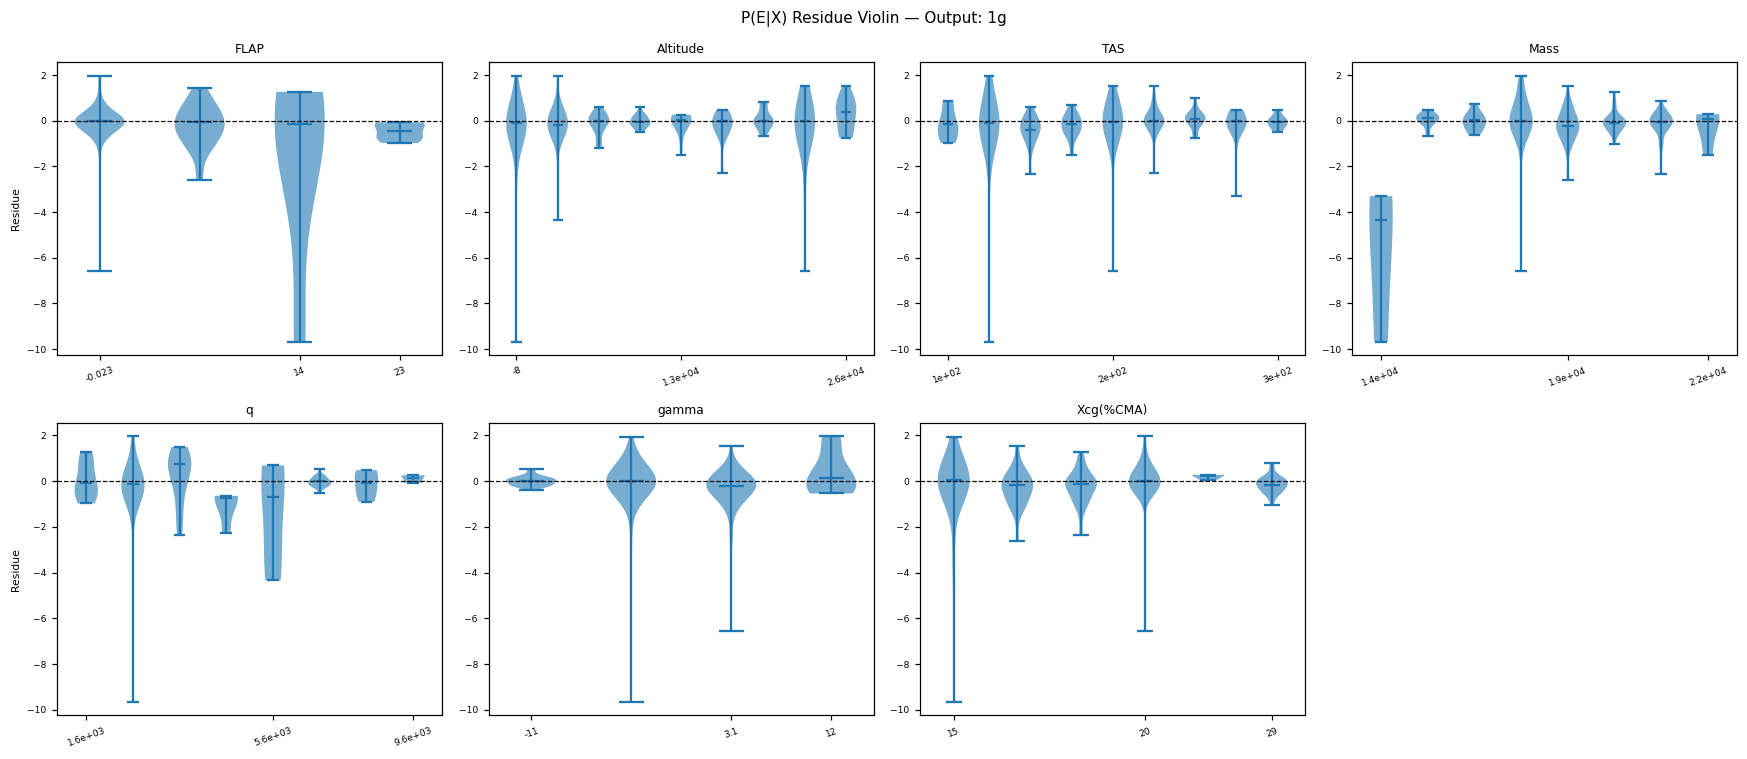
\includegraphics[width=1.0\linewidth,height=0.80\textheight,keepaspectratio]{analysis_plots/pex_violin_res_1g.png}\end{center}
\end{minipage}\par\medskip
\par\begin{minipage}{\linewidth}
\subsection*{\normalsize Residue --- Vertical maneuver}
\begin{center}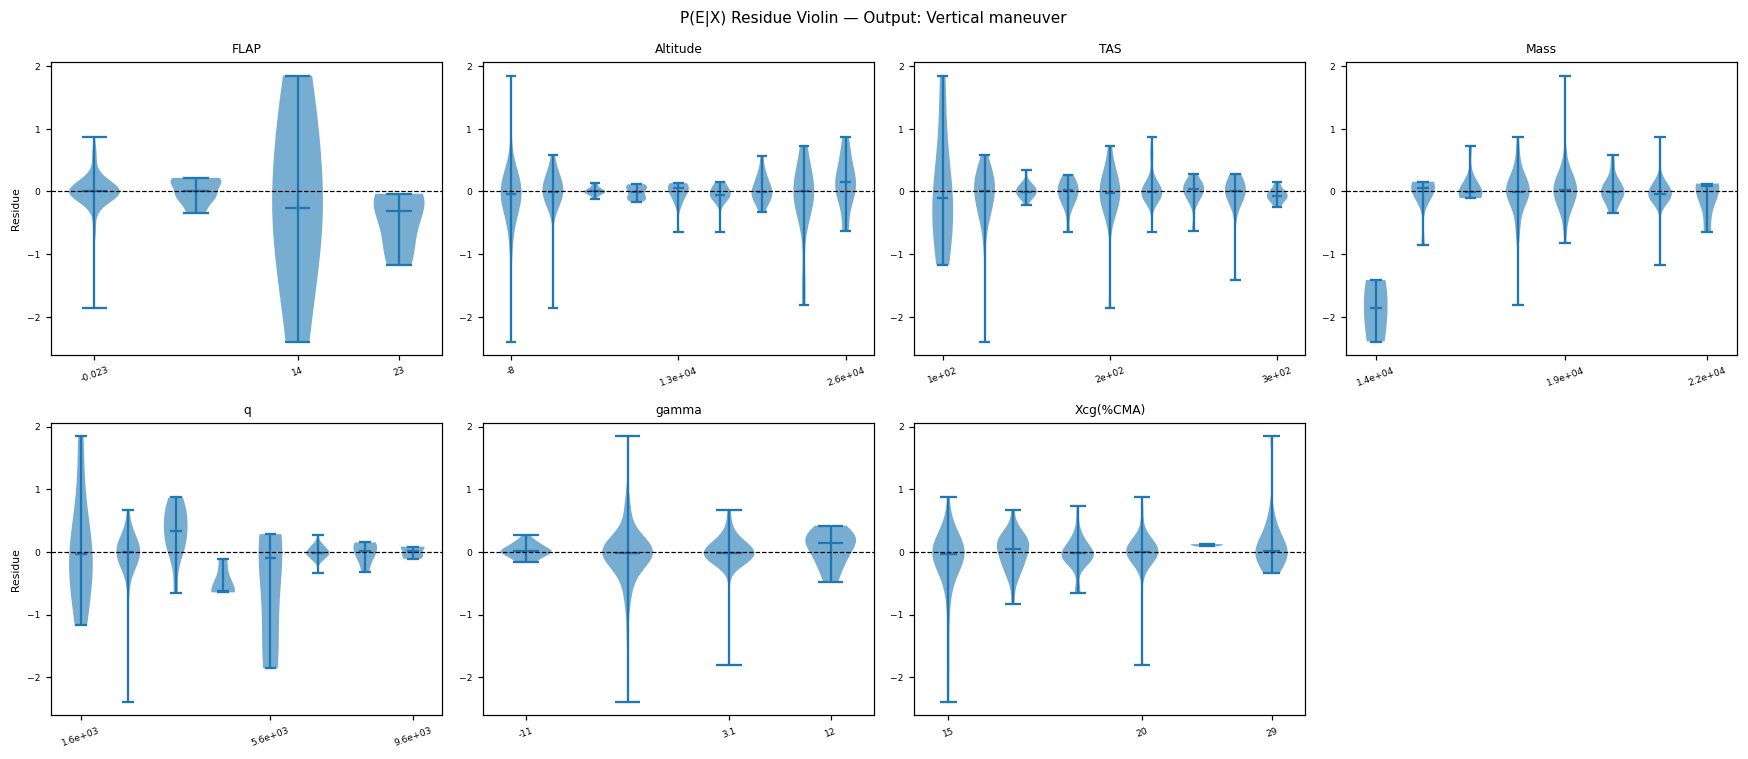
\includegraphics[width=1.0\linewidth,height=0.80\textheight,keepaspectratio]{analysis_plots/pex_violin_res_Vertical_maneuver.png}\end{center}
\end{minipage}\par\medskip
\par\begin{minipage}{\linewidth}
\subsection*{\normalsize Residue --- Vertical gust}
\begin{center}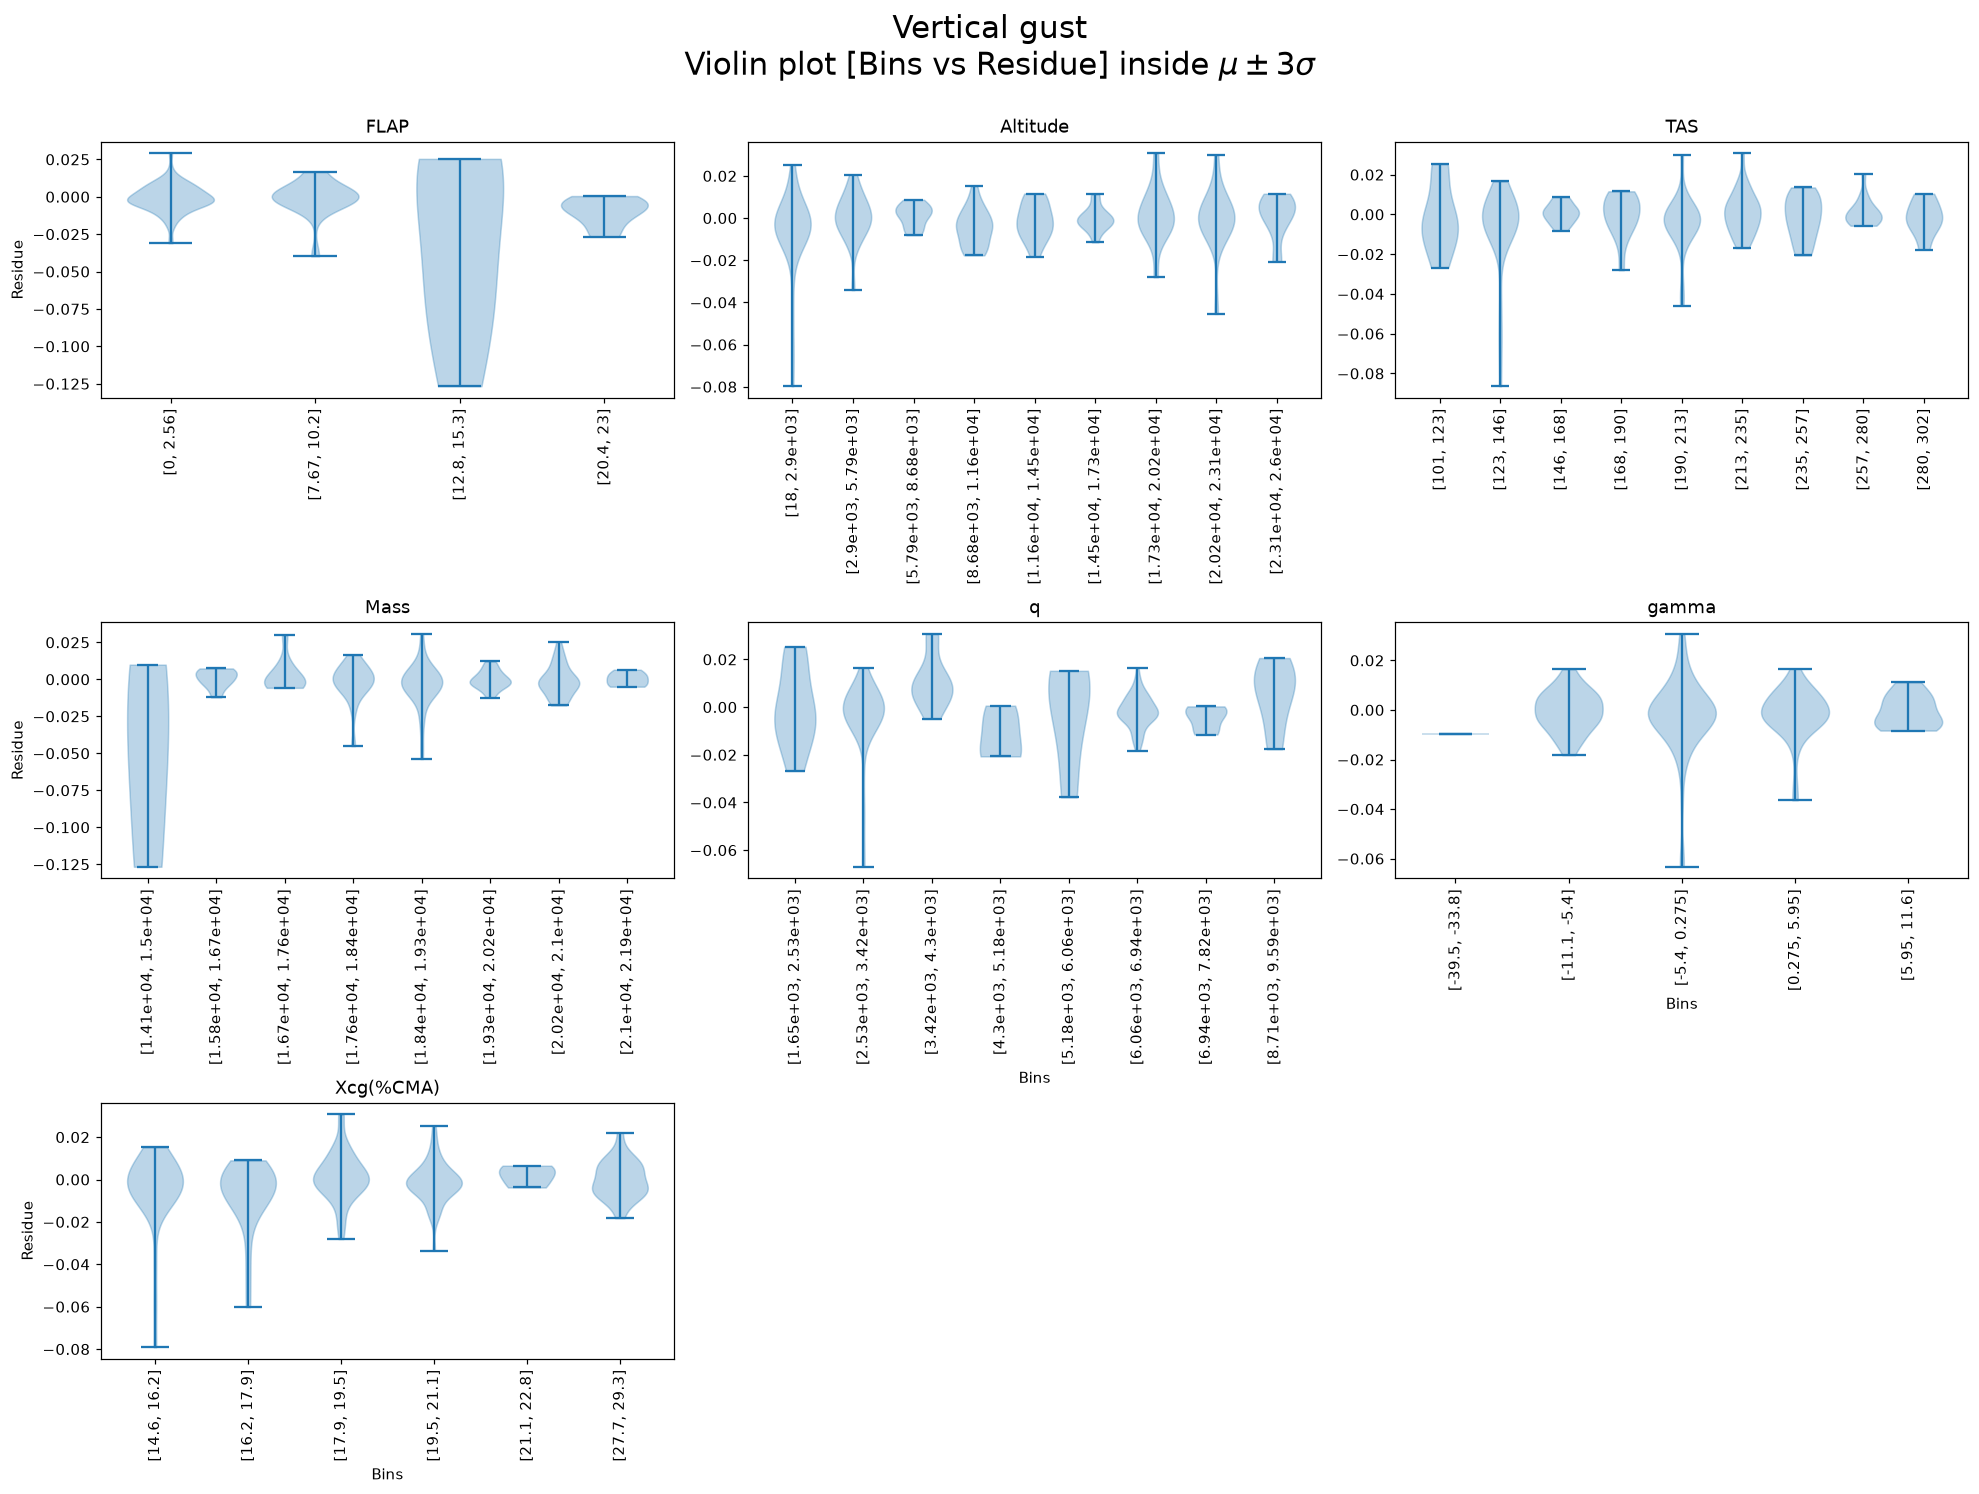
\includegraphics[width=1.0\linewidth,height=0.80\textheight,keepaspectratio]{analysis_plots/pex_violin_res_Vertical_gust.png}\end{center}
\end{minipage}\par\medskip
\par\begin{minipage}{\linewidth}
\subsection*{\normalsize Residue --- Turn}
\begin{center}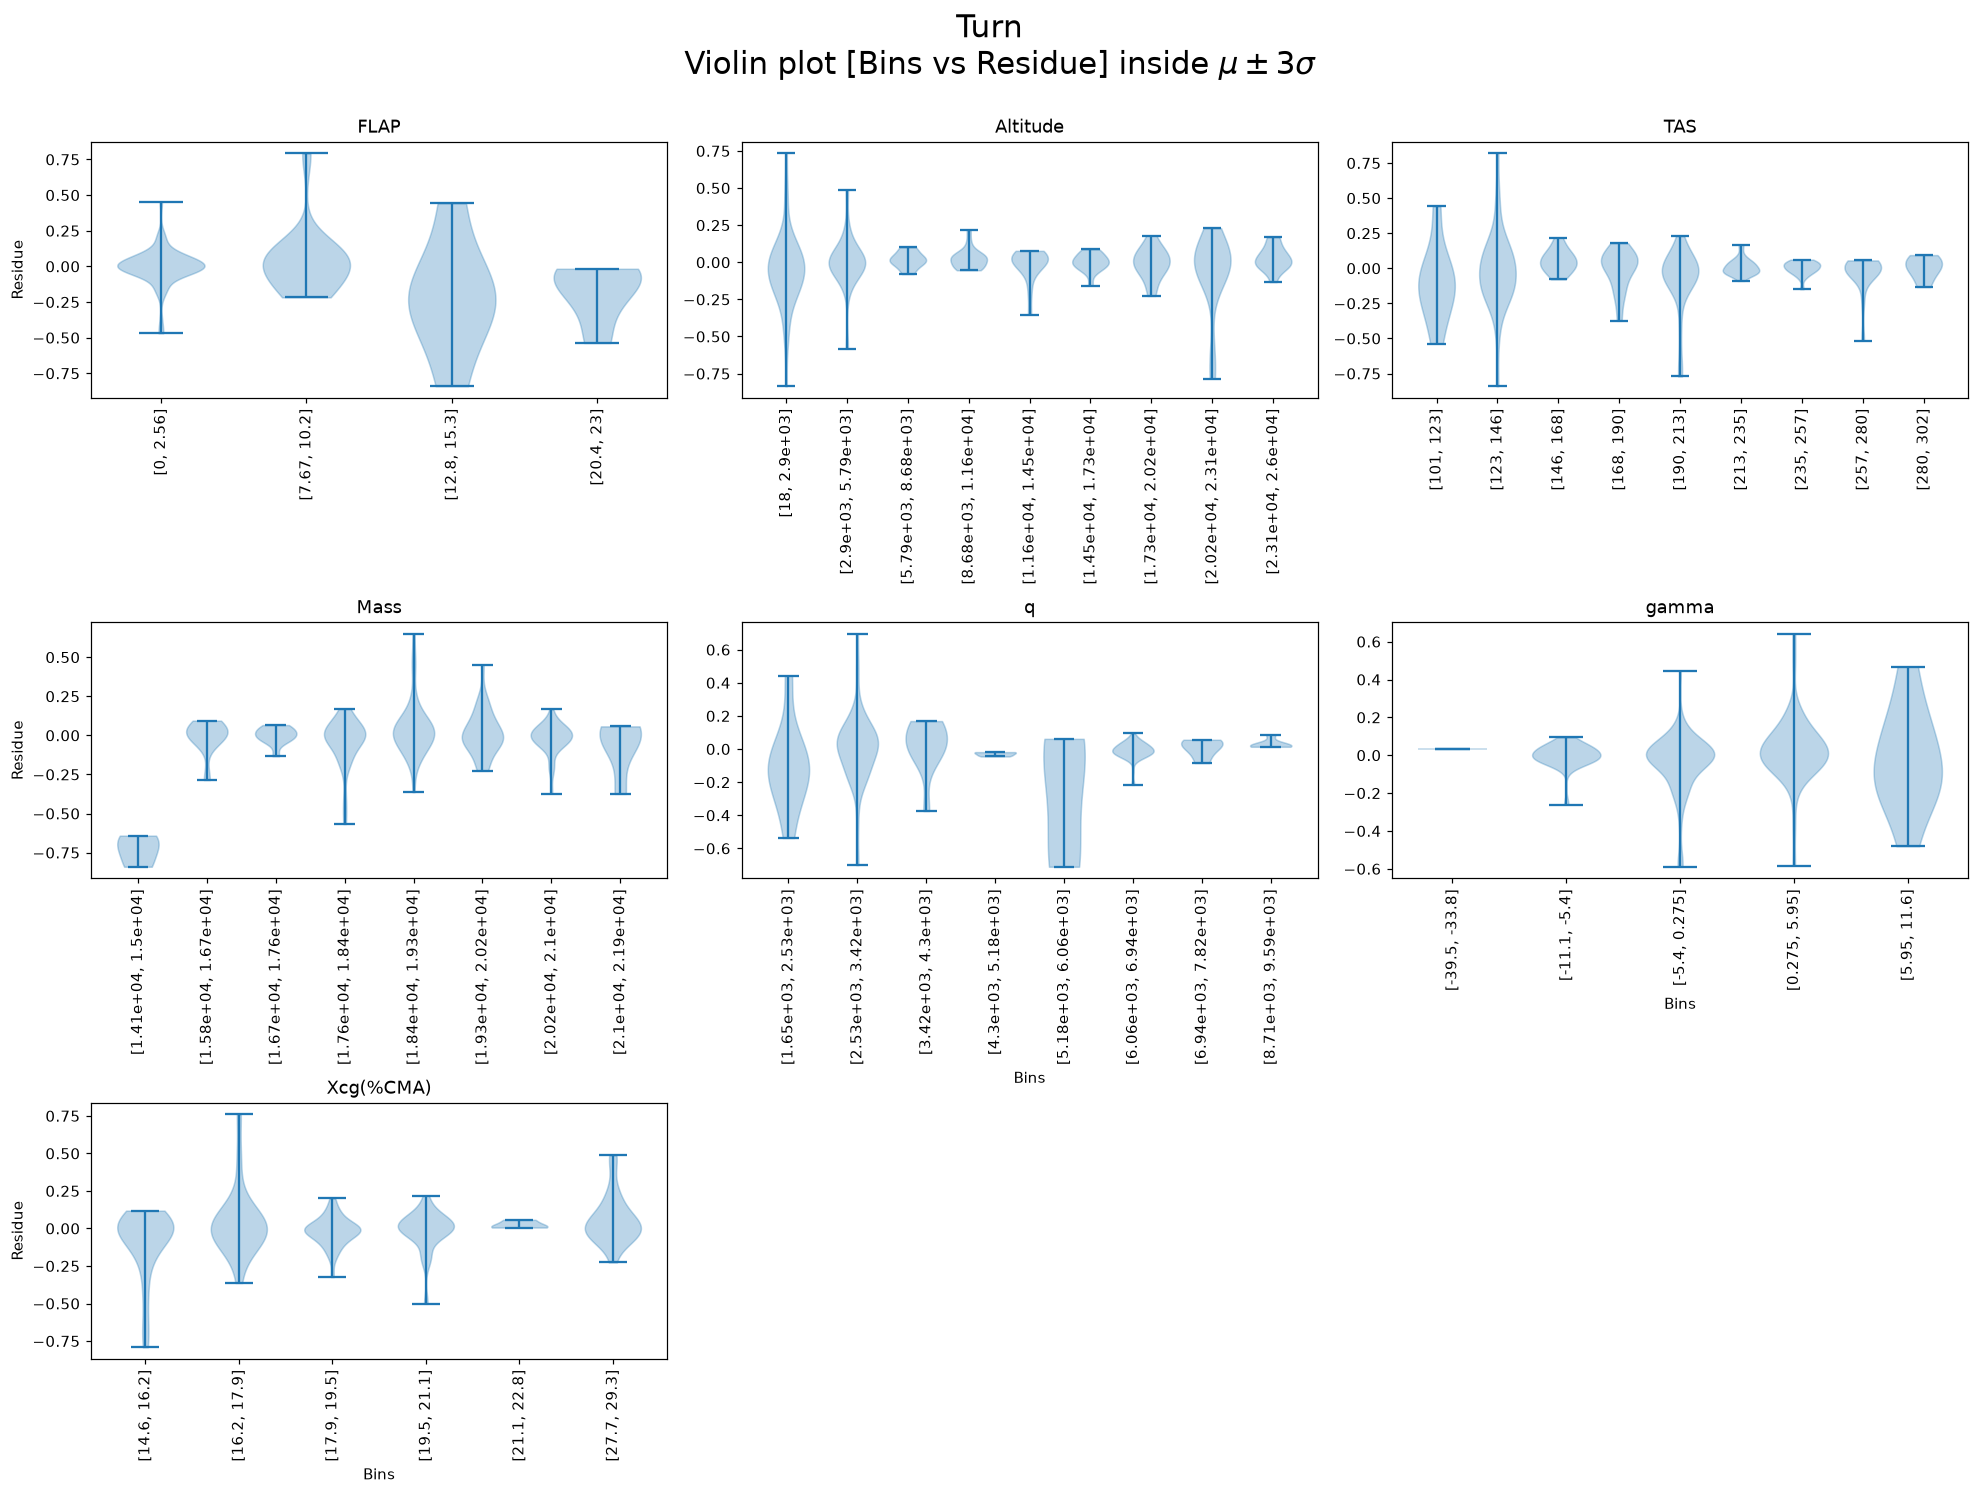
\includegraphics[width=1.0\linewidth,height=0.80\textheight,keepaspectratio]{analysis_plots/pex_violin_res_Turn.png}\end{center}
\end{minipage}\par\medskip
\par\begin{minipage}{\linewidth}
\subsection*{\normalsize Residue --- Frontal gust}
\begin{center}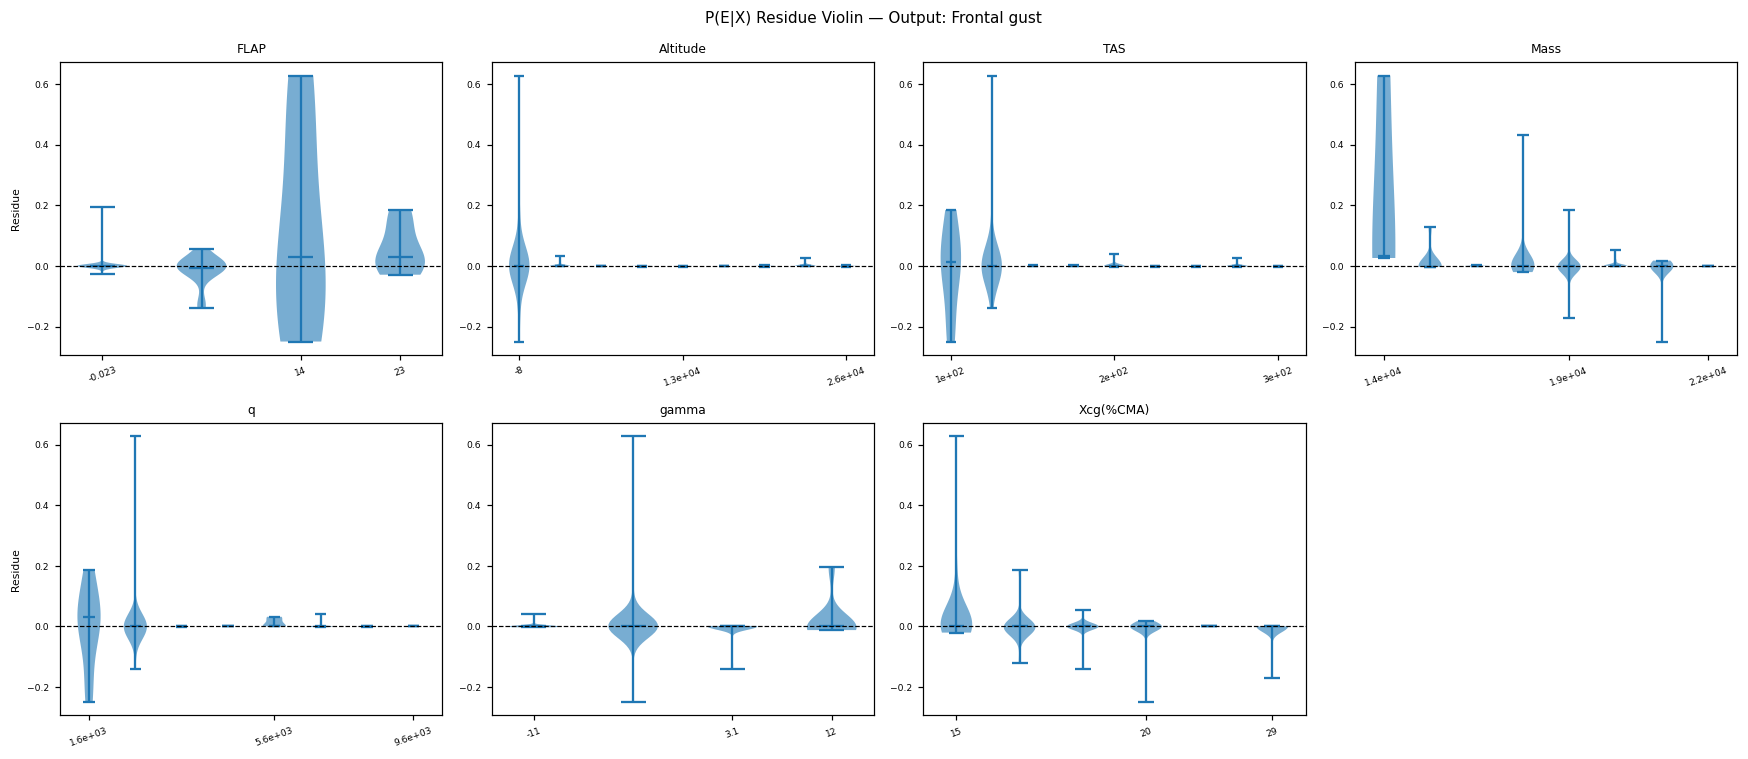
\includegraphics[width=1.0\linewidth,height=0.80\textheight,keepaspectratio]{analysis_plots/pex_violin_res_Frontal_gust.png}\end{center}
\end{minipage}\par\medskip
\par\begin{minipage}{\linewidth}
\subsection*{\normalsize Residue --- n0}
\begin{center}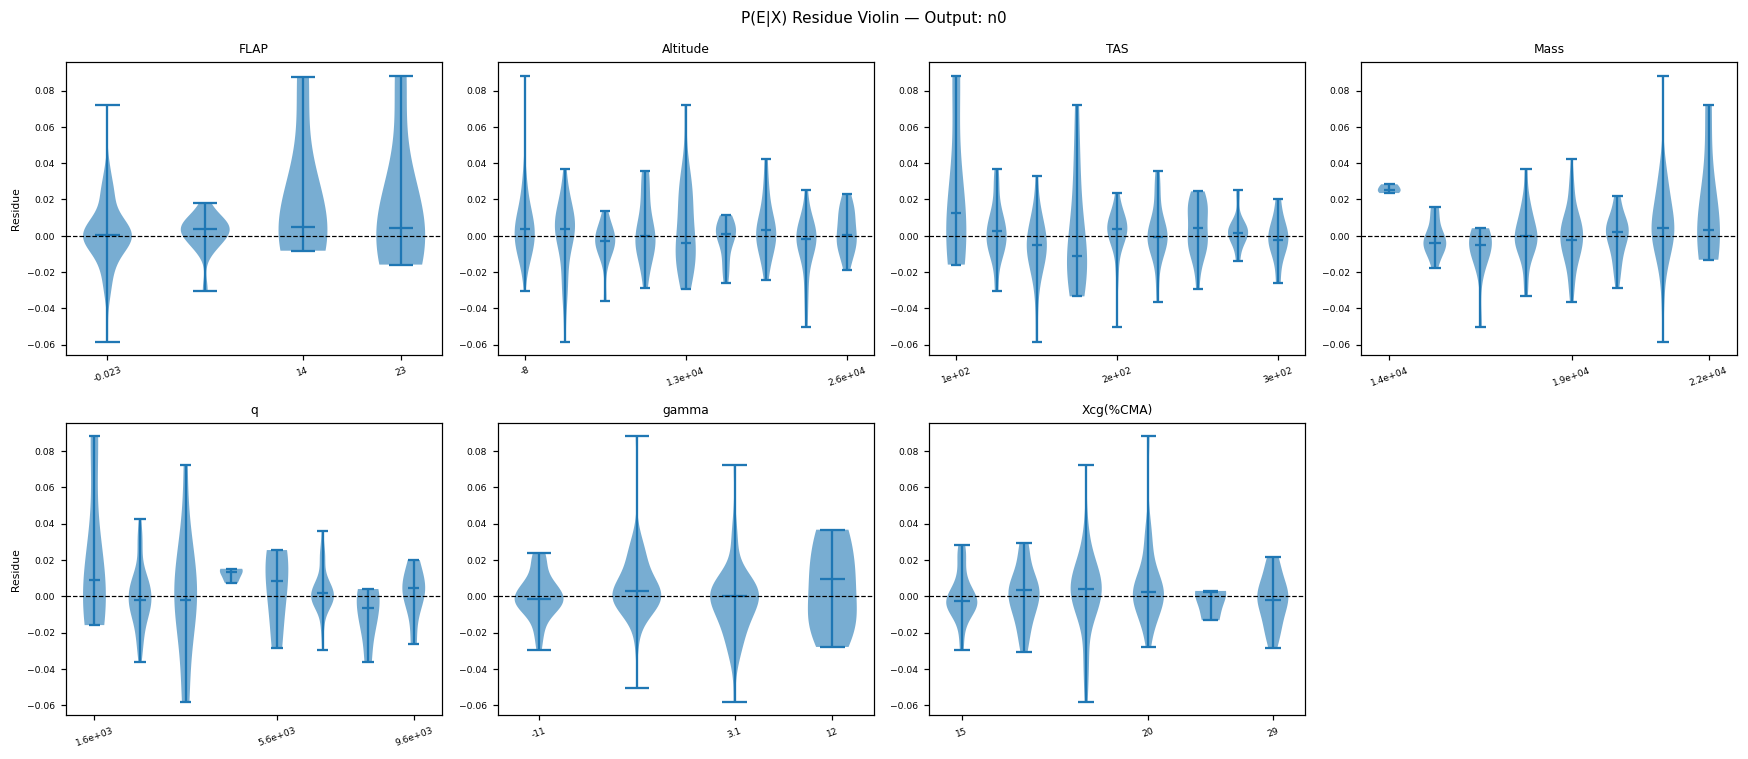
\includegraphics[width=1.0\linewidth,height=0.80\textheight,keepaspectratio]{analysis_plots/pex_violin_res_n0.png}\end{center}
\end{minipage}\par\medskip
\par\begin{minipage}{\linewidth}
\subsection*{\normalsize Residue --- Giro}
\begin{center}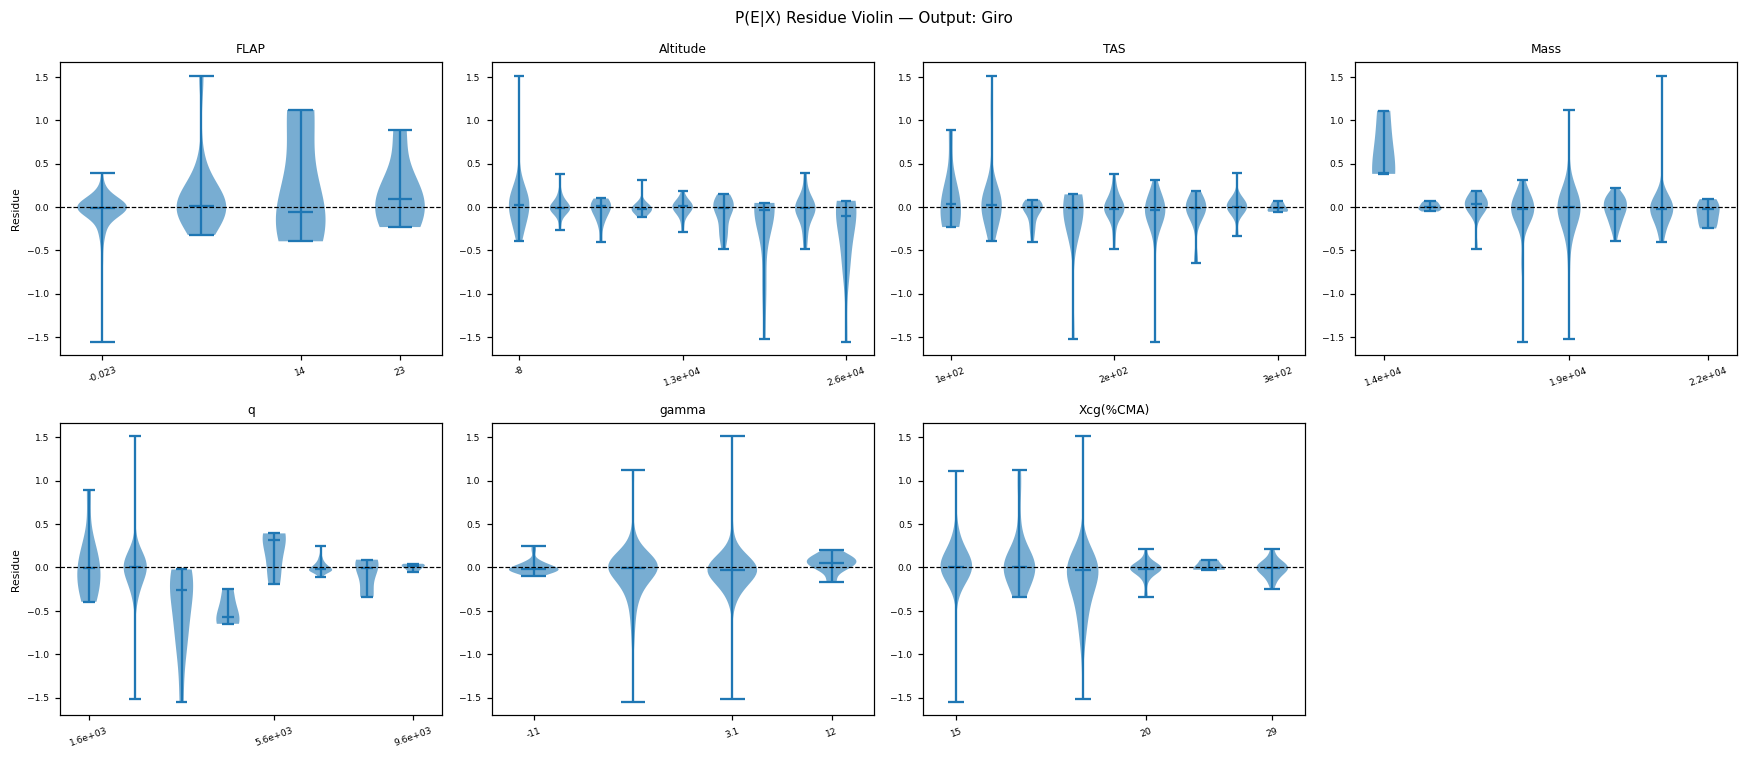
\includegraphics[width=1.0\linewidth,height=0.80\textheight,keepaspectratio]{analysis_plots/pex_violin_res_Giro.png}\end{center}
\end{minipage}\par\medskip
\clearpage
\exhead{Absolute Error Violin Plots per Output (binned by input)}
\par\begin{minipage}{\linewidth}
\subsection*{\normalsize Absolute Error --- 1g}
\begin{center}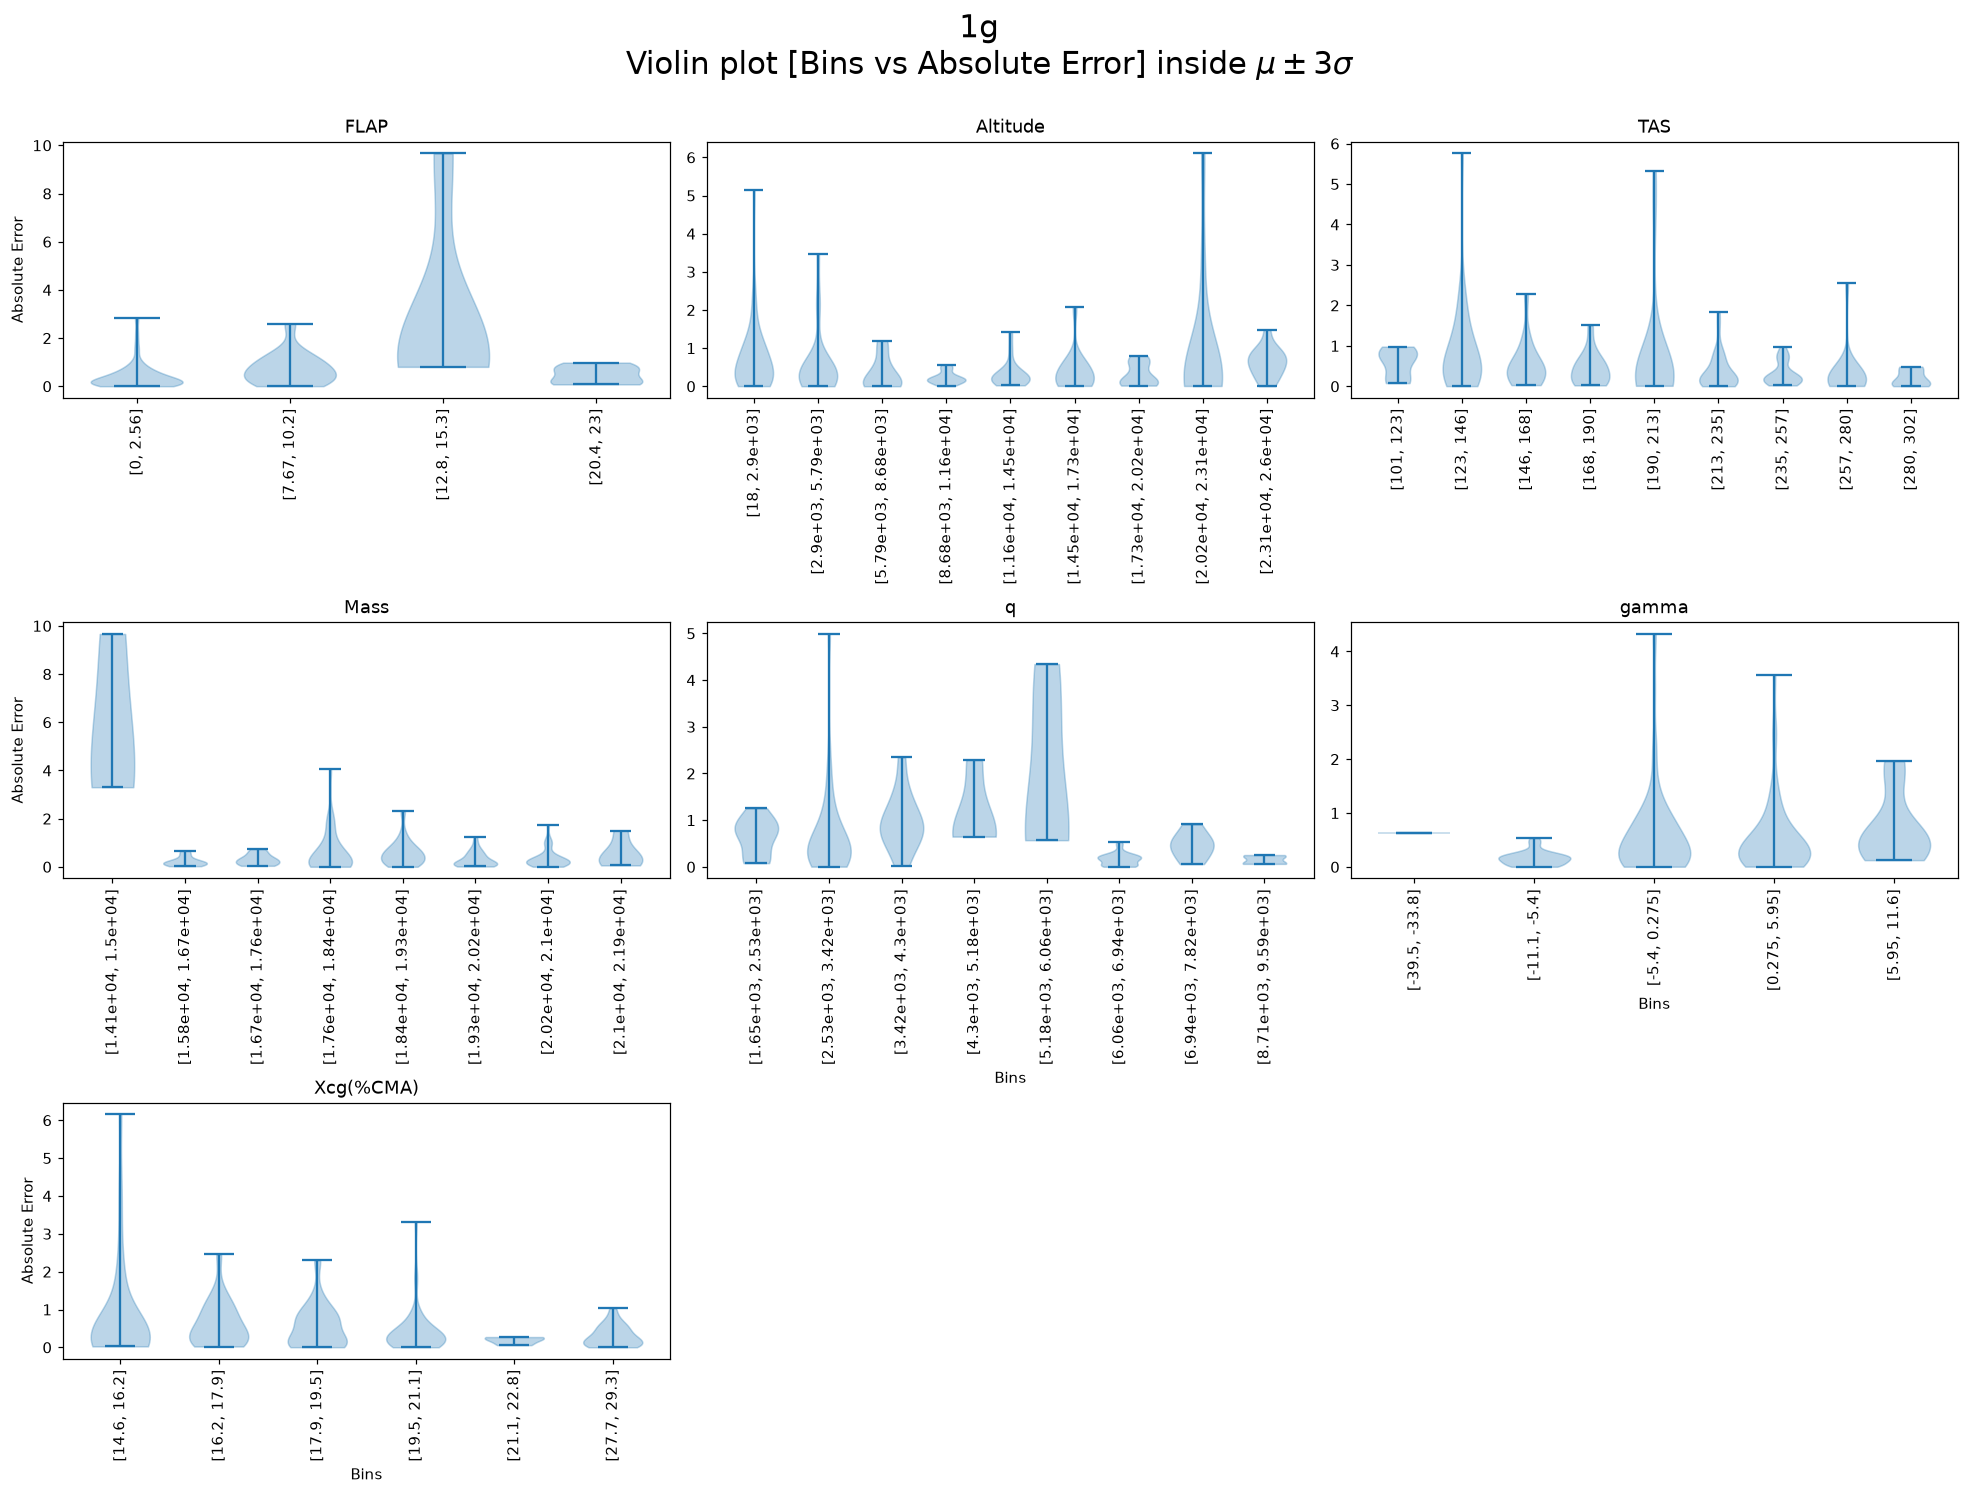
\includegraphics[width=1.0\linewidth,height=0.80\textheight,keepaspectratio]{analysis_plots/pex_violin_abs_1g.png}\end{center}
\end{minipage}\par\medskip
\par\begin{minipage}{\linewidth}
\subsection*{\normalsize Absolute Error --- Vertical maneuver}
\begin{center}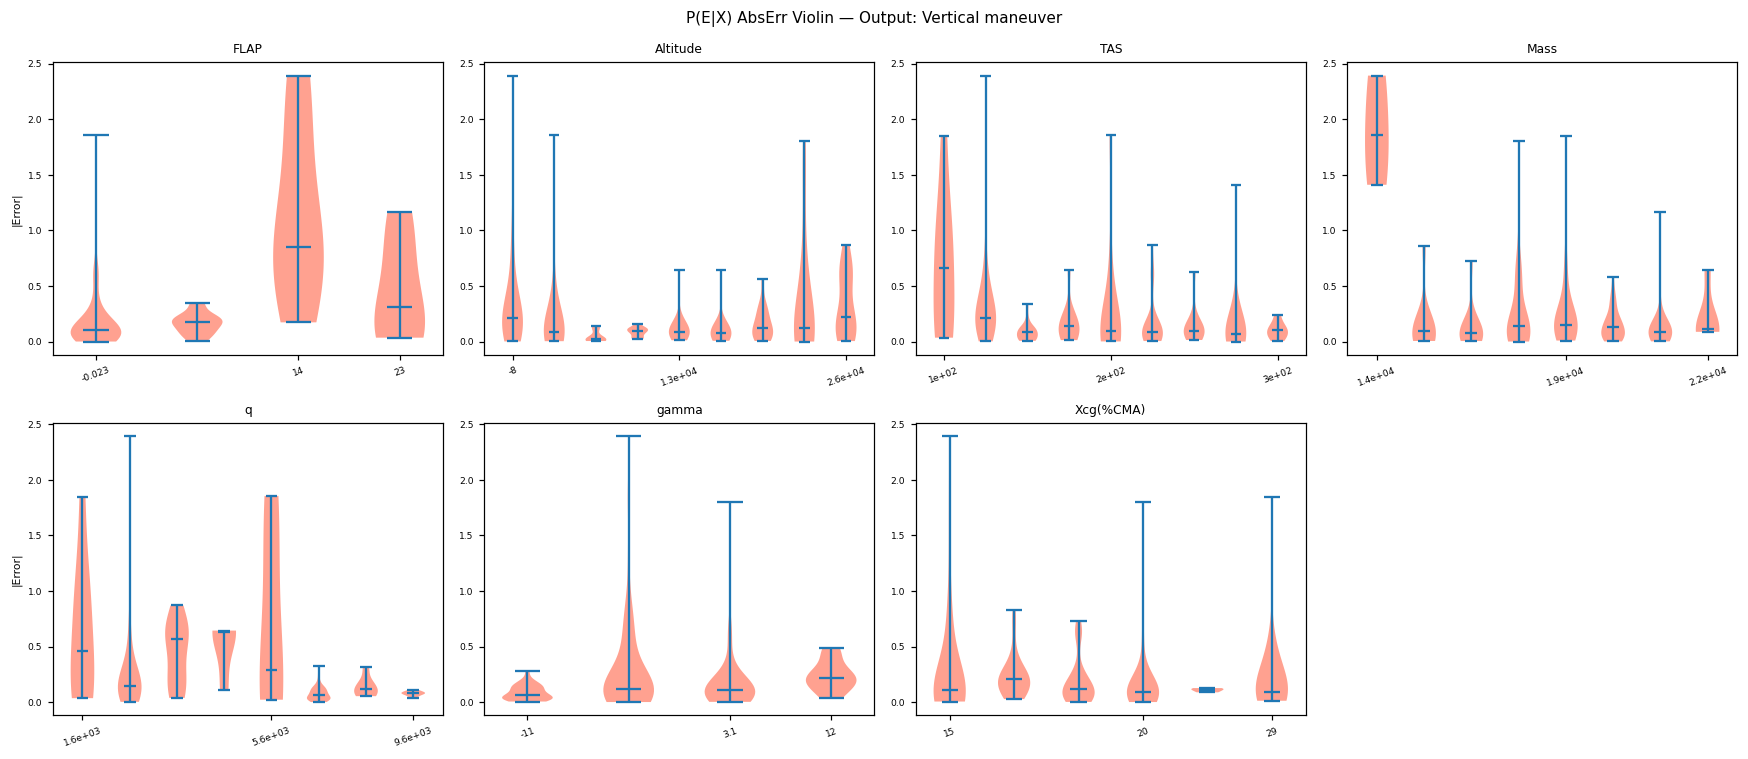
\includegraphics[width=1.0\linewidth,height=0.80\textheight,keepaspectratio]{analysis_plots/pex_violin_abs_Vertical_maneuver.png}\end{center}
\end{minipage}\par\medskip
\par\begin{minipage}{\linewidth}
\subsection*{\normalsize Absolute Error --- Vertical gust}
\begin{center}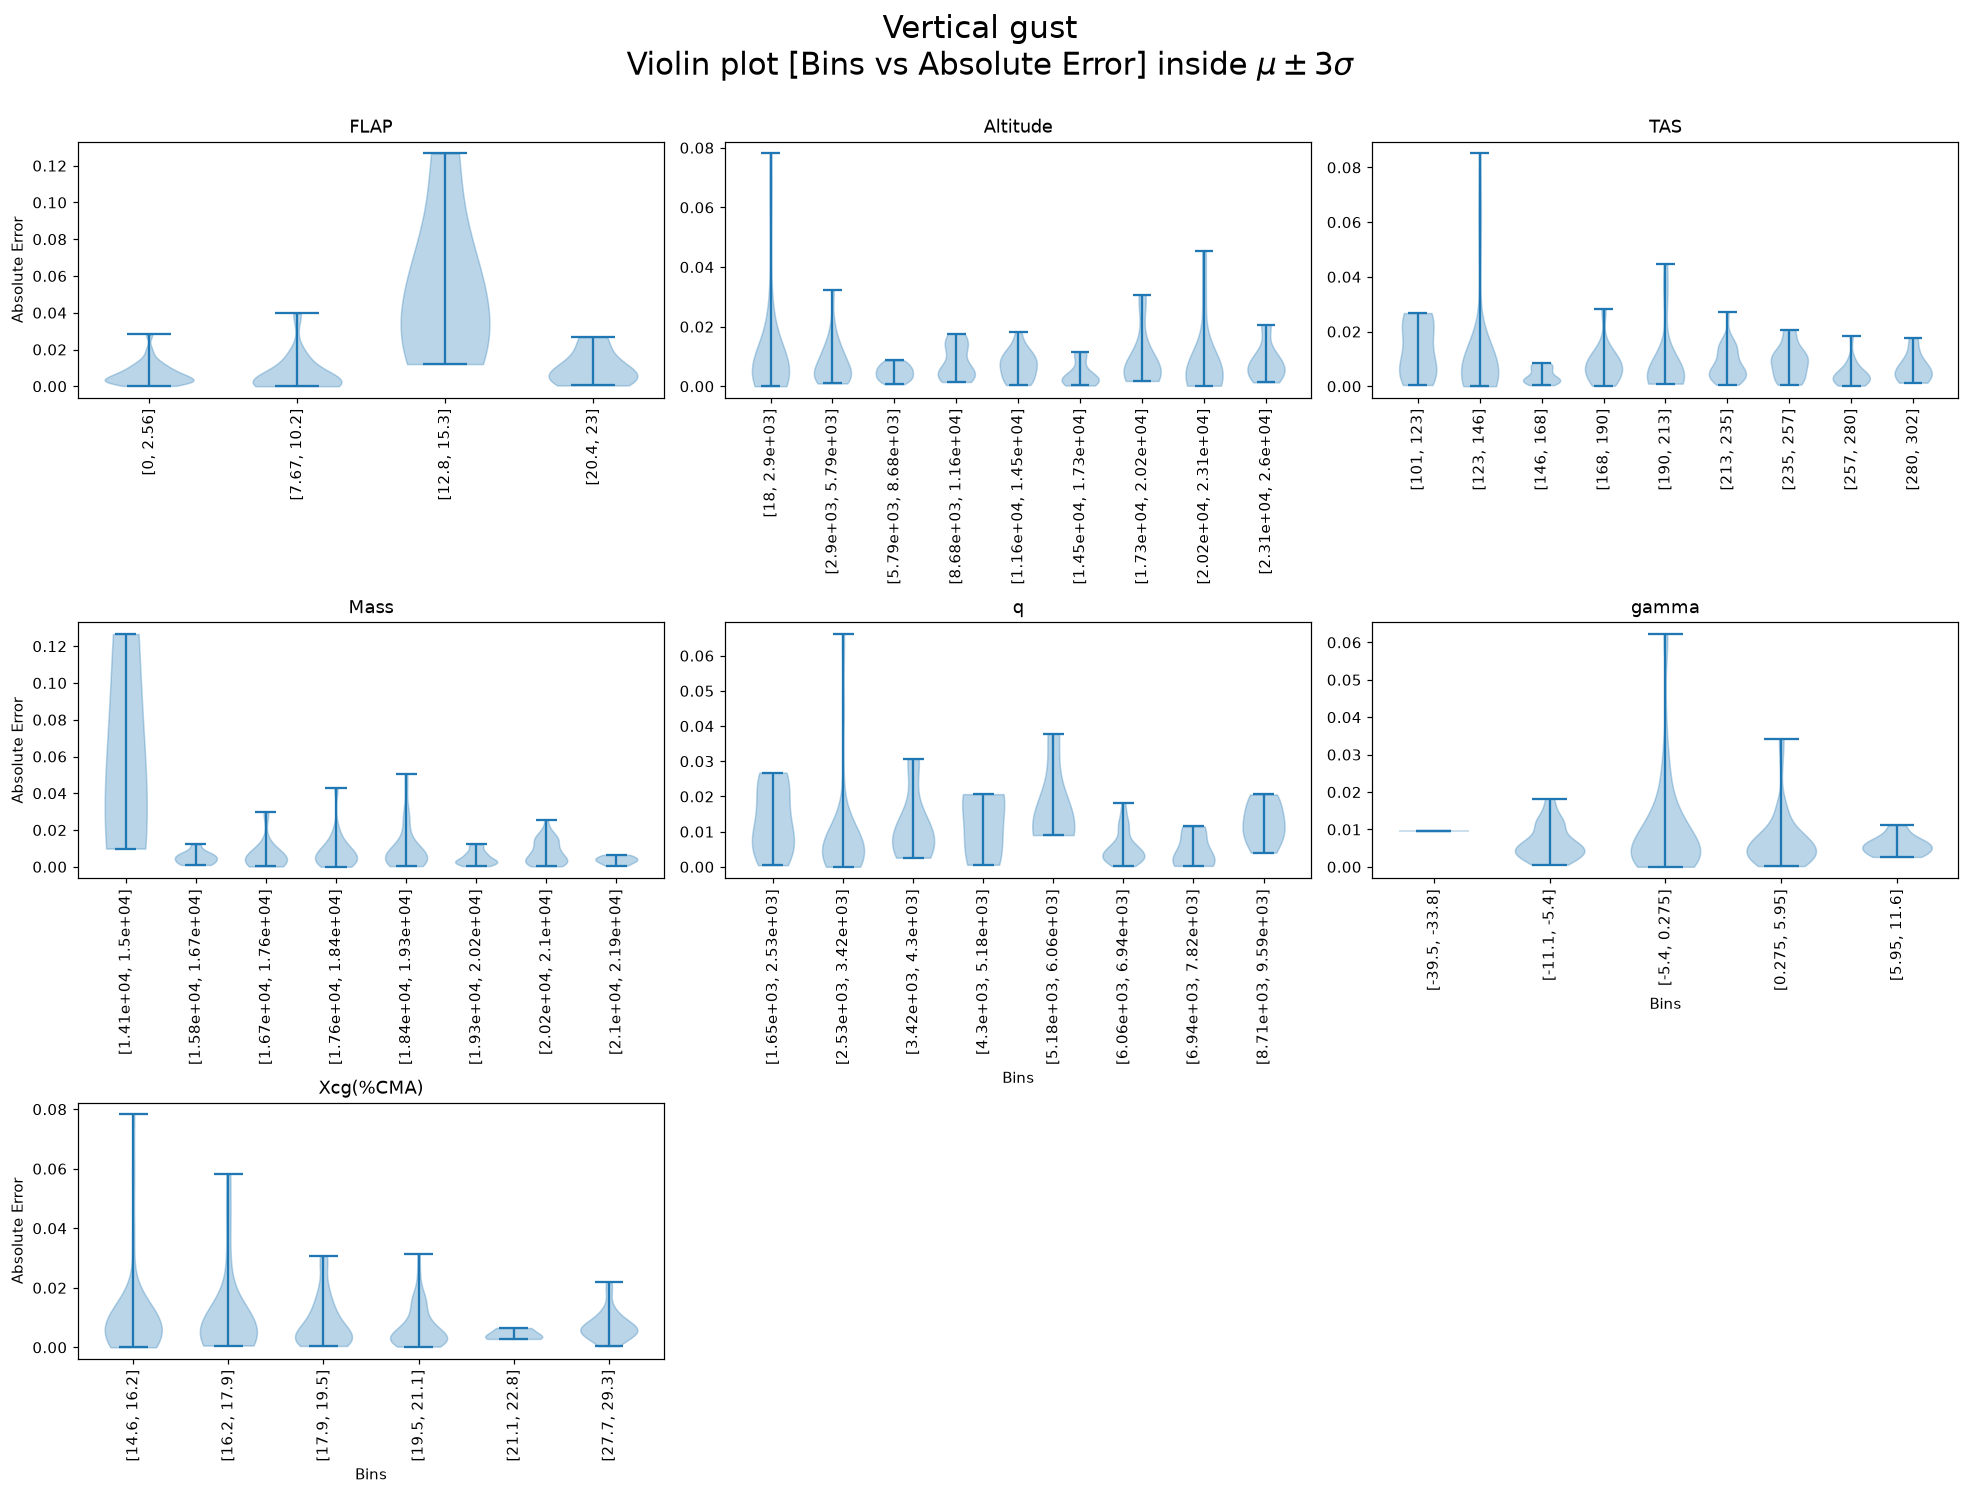
\includegraphics[width=1.0\linewidth,height=0.80\textheight,keepaspectratio]{analysis_plots/pex_violin_abs_Vertical_gust.png}\end{center}
\end{minipage}\par\medskip
\par\begin{minipage}{\linewidth}
\subsection*{\normalsize Absolute Error --- Turn}
\begin{center}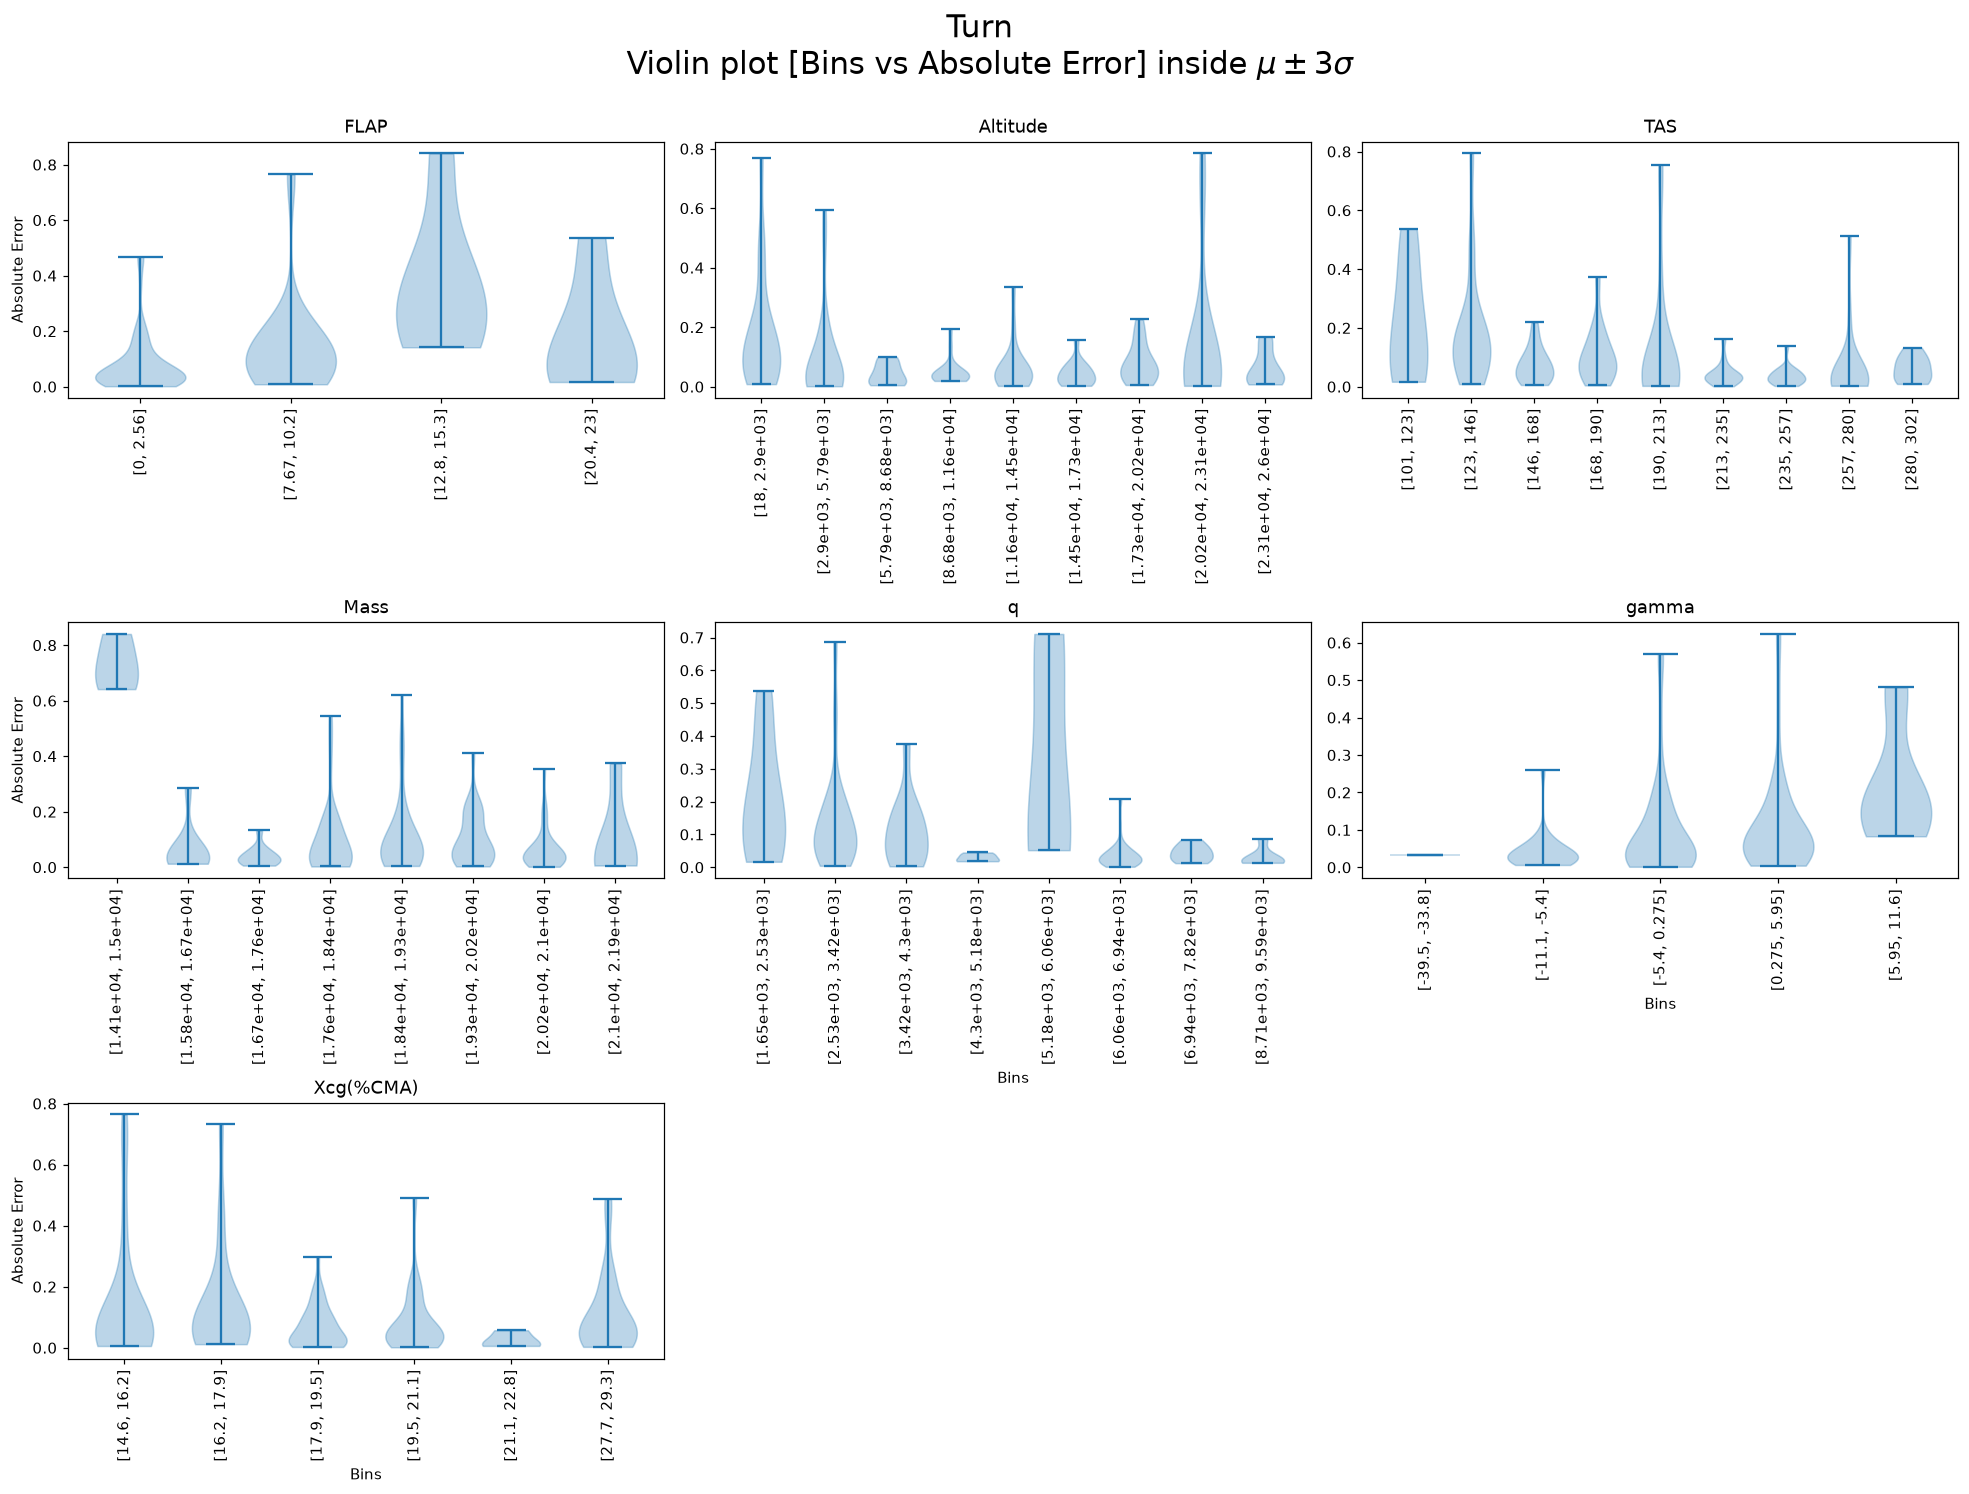
\includegraphics[width=1.0\linewidth,height=0.80\textheight,keepaspectratio]{analysis_plots/pex_violin_abs_Turn.png}\end{center}
\end{minipage}\par\medskip
\par\begin{minipage}{\linewidth}
\subsection*{\normalsize Absolute Error --- Frontal gust}
\begin{center}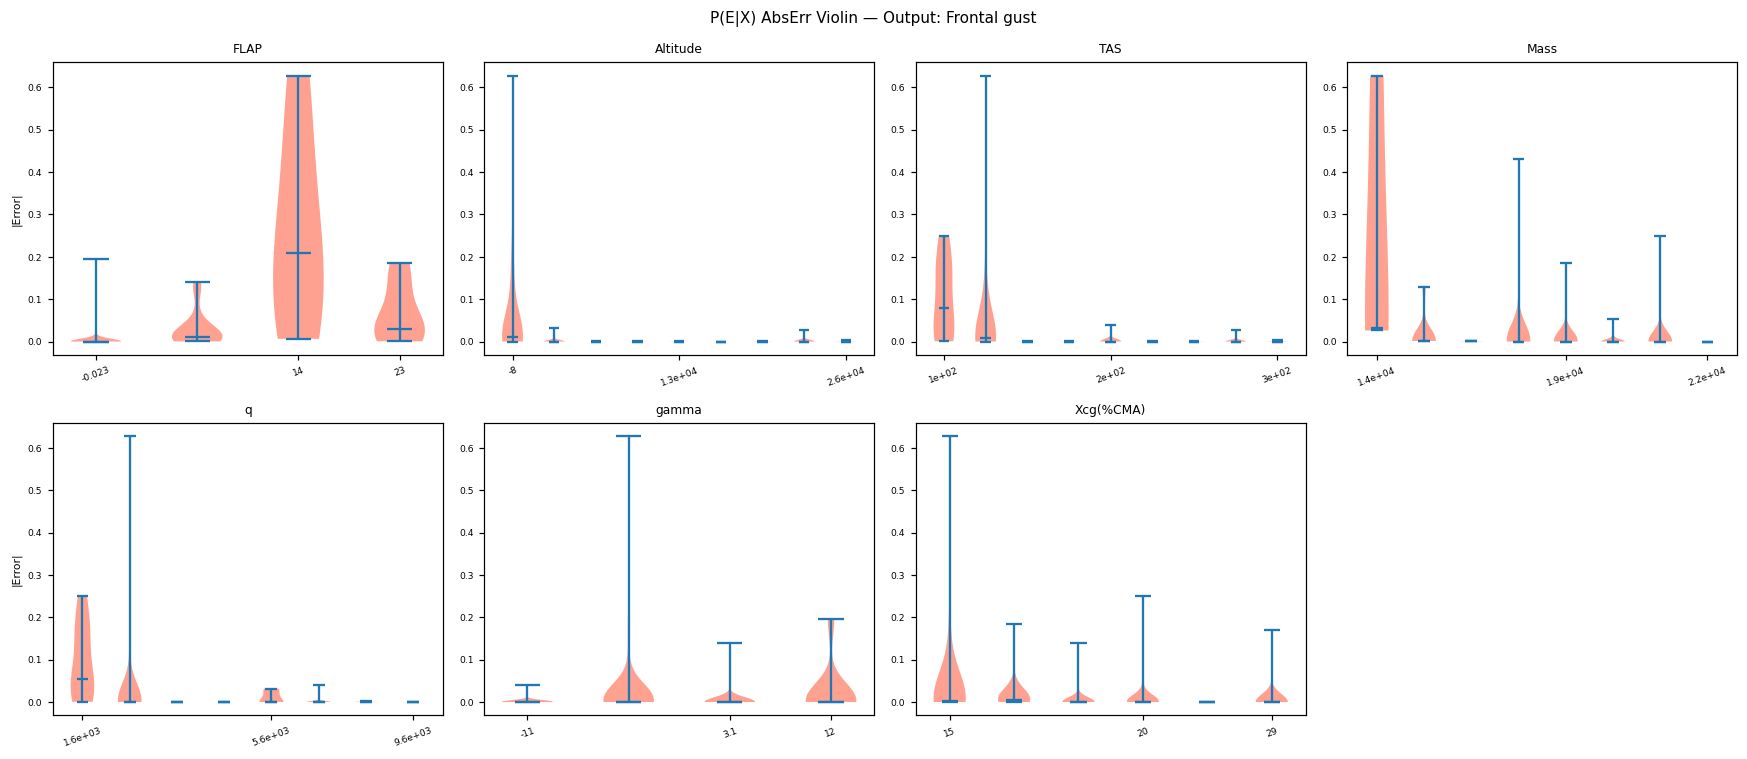
\includegraphics[width=1.0\linewidth,height=0.80\textheight,keepaspectratio]{analysis_plots/pex_violin_abs_Frontal_gust.png}\end{center}
\end{minipage}\par\medskip
\par\begin{minipage}{\linewidth}
\subsection*{\normalsize Absolute Error --- n0}
\begin{center}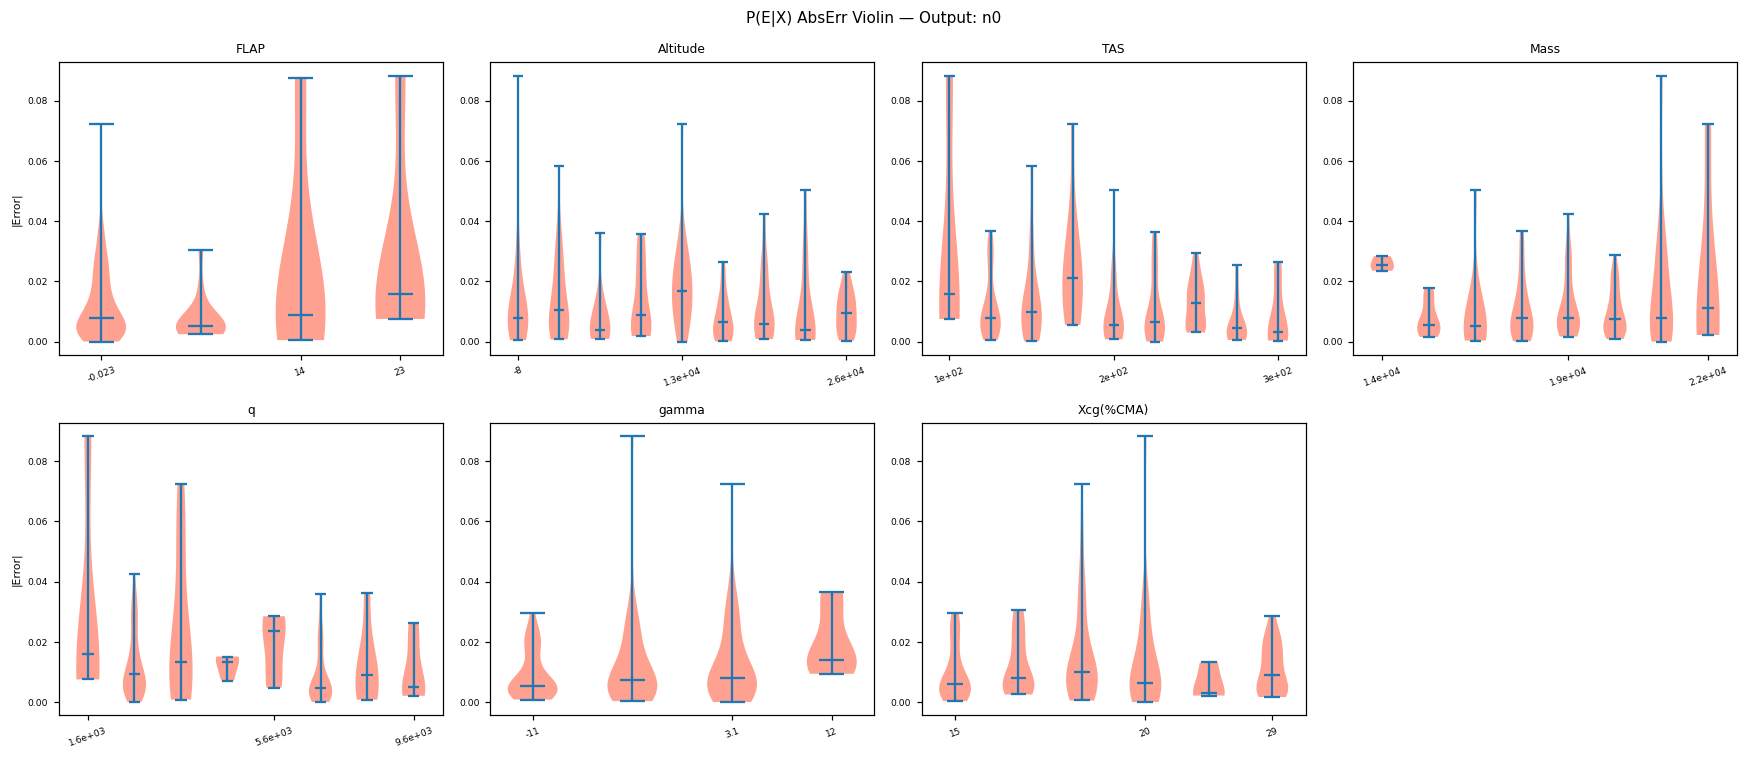
\includegraphics[width=1.0\linewidth,height=0.80\textheight,keepaspectratio]{analysis_plots/pex_violin_abs_n0.png}\end{center}
\end{minipage}\par\medskip
\par\begin{minipage}{\linewidth}
\subsection*{\normalsize Absolute Error --- Giro}
\begin{center}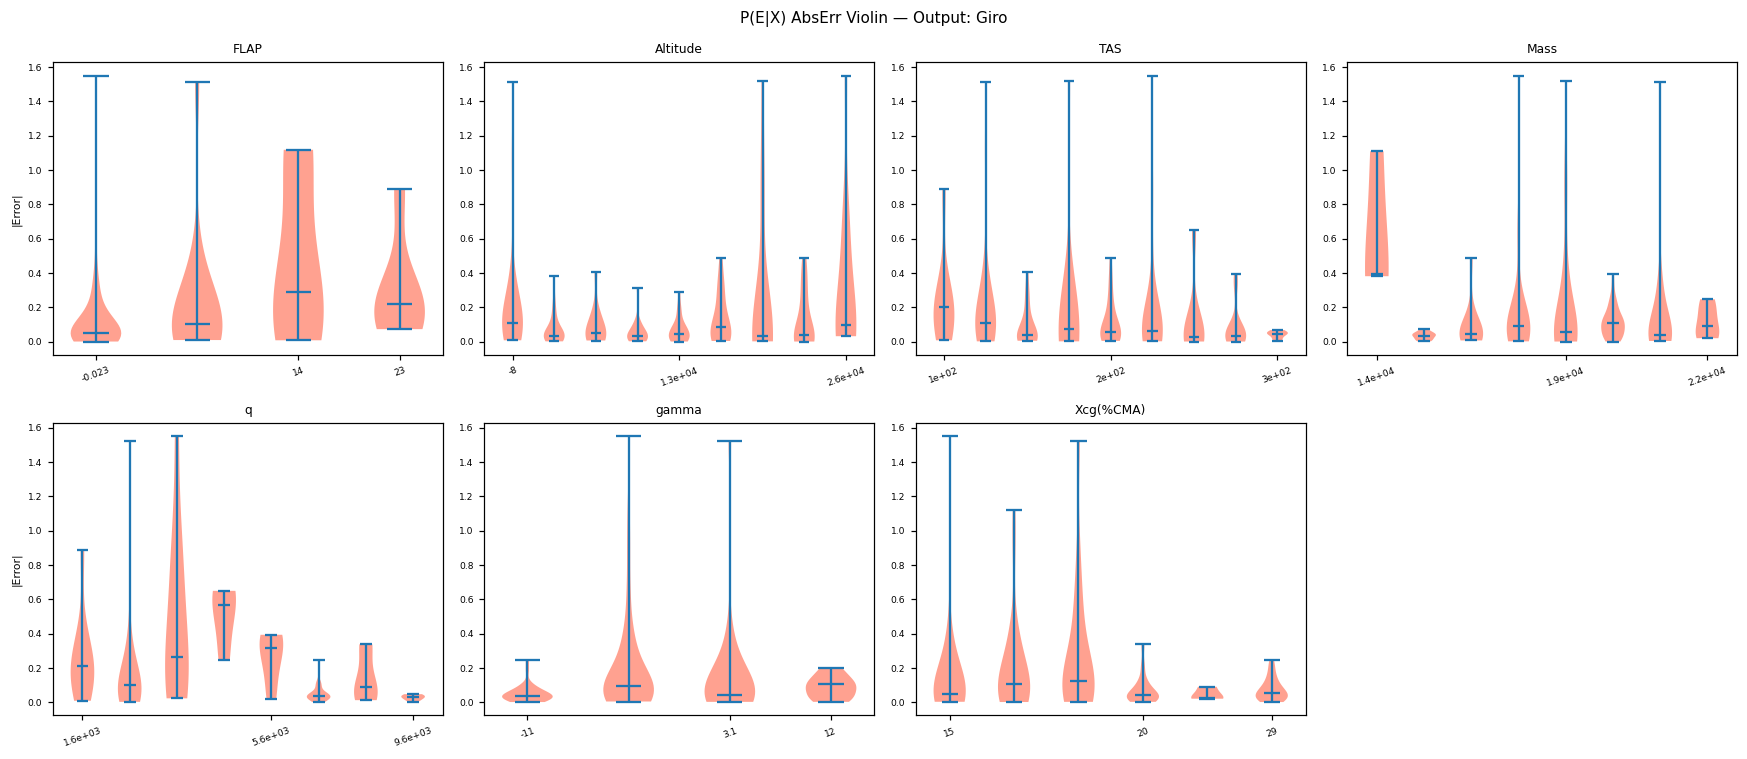
\includegraphics[width=1.0\linewidth,height=0.80\textheight,keepaspectratio]{analysis_plots/pex_violin_abs_Giro.png}\end{center}
\end{minipage}\par\medskip
\clearpage
\section{P(E|Y) --- Error Conditional on Outputs}
\label{sec:d5}

We study whether the error depends on the output magnitude. A significant trend (Pearson or Spearman $p<0.05$) means the model is more accurate in some output ranges than others --- a form of heteroscedasticity.

\par\begin{minipage}{\linewidth}
\exhead{Residue vs True Output --- Scatter}
The legend shows the least-squares fit and its R\textsuperscript{2}.
\begin{center}
\includegraphics[width=1.0\linewidth,height=0.80\textheight,keepaspectratio]{analysis_plots/pey_residue_scatter.png}\end{center}
\end{minipage}\par\medskip
\par\begin{minipage}{\linewidth}
\exhead{Residue Trend Tests (Pearson / Spearman)}
Each output's residue against its own true value, as the extended validation notebook computes them: correlation coefficient, trend-test p-value ($p<0.05$ = significant trend) and, for Pearson, the normalized slope. The full cross-output tables are in the extended validation HTML.
\begin{center}
\footnotesize
\renewcommand{\arraystretch}{1.15}
\resizebox{\linewidth}{!}{%
\begin{tabular}{|l|r|r|r|r|r|r|r|}
\hline
\textbf{} & \textbf{1g} & \textbf{Vertical maneuver} & \textbf{Vertical gust} & \textbf{Turn} & \textbf{Frontal gust} & \textbf{n0} & \textbf{Giro} \\ \hline
\textbf{Pearson coeff.} & 0.2648 & 0.2798 & 0.1437 & 0.4969 & 0.201 & 0.2437 & 0.4019 \\ \hline
\textbf{p-value} & 0.000413 & 0.000184 & 0.0584 & 3.08e-12 & 0.0078 & 0.0012 & 3.88e-08 \\ \hline
\textbf{Slope (normalized)} & 0.133 & 0.1357 & 0.0621 & 0.2616 & 0.0511 & 0.1641 & 0.2025 \\ \hline
\end{tabular}
}
\par\vspace{2pt}
{\scriptsize Residue vs.\ its true output --- Pearson trend test}
\end{center}
\begin{center}
\footnotesize
\renewcommand{\arraystretch}{1.15}
\resizebox{\linewidth}{!}{%
\begin{tabular}{|l|r|r|r|r|r|r|r|}
\hline
\textbf{} & \textbf{1g} & \textbf{Vertical maneuver} & \textbf{Vertical gust} & \textbf{Turn} & \textbf{Frontal gust} & \textbf{n0} & \textbf{Giro} \\ \hline
\textbf{Spearman coeff.} & 0.2005 & 0.1391 & 0.0809 & 0.309 & 0.1228 & 0.2224 & 0.2591 \\ \hline
\textbf{p-value} & 0.008 & 0.0671 & 0.2885 & 3.34e-05 & 0.1064 & 0.0032 & 0.000557 \\ \hline
\end{tabular}
}
\par\vspace{2pt}
{\scriptsize Residue vs.\ its true output --- Spearman trend test}
\end{center}
\end{minipage}\par\medskip
\par\begin{minipage}{\linewidth}
\exhead{Residue Violin vs True Output Bins}
Bins determined by Sturges rule. Median line dashed at 0.
\begin{center}
\includegraphics[width=1.0\linewidth,height=0.80\textheight,keepaspectratio]{analysis_plots/pey_residue_violin.png}\end{center}
\end{minipage}\par\medskip
\par\begin{minipage}{\linewidth}
\exhead{Absolute Error vs True Output --- Scatter}
The legend shows the least-squares fit and its R\textsuperscript{2}.
\begin{center}
\includegraphics[width=1.0\linewidth,height=0.80\textheight,keepaspectratio]{analysis_plots/pey_abserr_scatter.png}\end{center}
\end{minipage}\par\medskip
\par\begin{minipage}{\linewidth}
\exhead{Absolute Error Trend Tests (Pearson / Spearman)}
\begin{center}
\footnotesize
\renewcommand{\arraystretch}{1.15}
\resizebox{\linewidth}{!}{%
\begin{tabular}{|l|r|r|r|r|r|r|r|}
\hline
\textbf{} & \textbf{1g} & \textbf{Vertical maneuver} & \textbf{Vertical gust} & \textbf{Turn} & \textbf{Frontal gust} & \textbf{n0} & \textbf{Giro} \\ \hline
\textbf{Pearson coeff.} & -0.4003 & -0.4525 & -0.1635 & -0.3047 & 0.4101 & 0.085 & 0.2437 \\ \hline
\textbf{p-value} & 4.44e-08 & 3.65e-10 & 0.0311 & 4.36e-05 & 1.91e-08 & 0.2648 & 0.0012 \\ \hline
\textbf{Slope (normalized)} & -0.2151 & -0.3276 & -0.0738 & -0.2603 & 0.1421 & 0.0707 & 0.2099 \\ \hline
\end{tabular}
}
\par\vspace{2pt}
{\scriptsize Absolute error vs.\ its true output --- Pearson trend test}
\end{center}
\begin{center}
\footnotesize
\renewcommand{\arraystretch}{1.15}
\resizebox{\linewidth}{!}{%
\begin{tabular}{|l|r|r|r|r|r|r|r|}
\hline
\textbf{} & \textbf{1g} & \textbf{Vertical maneuver} & \textbf{Vertical gust} & \textbf{Turn} & \textbf{Frontal gust} & \textbf{n0} & \textbf{Giro} \\ \hline
\textbf{Spearman coeff.} & -0.3798 & -0.3457 & -0.0237 & -0.1531 & 0.5743 & 0.0841 & -0.0858 \\ \hline
\textbf{p-value} & 2.36e-07 & 2.98e-06 & 0.7565 & 0.0437 & 1.17e-16 & 0.2701 & 0.26 \\ \hline
\end{tabular}
}
\par\vspace{2pt}
{\scriptsize Absolute error vs.\ its true output --- Spearman trend test}
\end{center}
\end{minipage}\par\medskip
\par\begin{minipage}{\linewidth}
\exhead{Absolute Error Violin vs True Output Bins}
\begin{center}
\includegraphics[width=1.0\linewidth,height=0.80\textheight,keepaspectratio]{analysis_plots/pey_abserr_violin.png}\end{center}
\end{minipage}\par\medskip
\clearpage
\section{Uncertainty Analysis}
\label{sec:d6}

A global binned uncertainty model (95th percentile, right-tailed) is trained on the validation split of the absolute error and evaluated on the held-out test split, as in the extended validation notebook. Coverage is the proportion of test points whose error falls inside the predicted bound; it should be close to 95\%.

\par\begin{minipage}{\linewidth}
\exhead{Coverage Plot}
\begin{center}
\includegraphics[width=1.0\linewidth,height=0.80\textheight,keepaspectratio]{analysis_plots/uncertainty_coverage.png}\end{center}
\end{minipage}\par\medskip
\exhead{Coverage Table}
\begin{center}
\footnotesize
\renewcommand{\arraystretch}{1.15}
\resizebox{\linewidth}{!}{%
\begin{tabular}{|l|r|r|r|r|r|r|r|r|}
\hline
\textbf{} & \textbf{1g} & \textbf{Vertical maneuver} & \textbf{Vertical gust} & \textbf{Turn} & \textbf{Frontal gust} & \textbf{n0} & \textbf{Giro} & \textbf{TOTAL COV} \\ \hline
\textbf{Coverage} & 97.13 & 94.83 & 94.25 & 96.55 & 94.83 & 96.55 & 92.53 & \textemdash \\ \hline
\textbf{CI} & [93.42, 99.06] & [90.41, 97.61] & [89.68, 97.21] & [92.65, 98.72] & [90.41, 97.61] & [92.65, 98.72] & [87.56, 95.96] & \textemdash \\ \hline
\end{tabular}
}
\par\vspace{2pt}
{\scriptsize Empirical coverage of the 95th-percentile uncertainty bound on the test split.}
\end{center}

\end{document}
